\documentclass[twoside]{book}

% Packages required by doxygen
\usepackage{fixltx2e}
\usepackage{calc}
\usepackage{doxygen}
\usepackage[export]{adjustbox} % also loads graphicx
\usepackage{graphicx}
\usepackage[utf8]{inputenc}
\usepackage{makeidx}
\usepackage{multicol}
\usepackage{multirow}
\PassOptionsToPackage{warn}{textcomp}
\usepackage{textcomp}
\usepackage[nointegrals]{wasysym}
\usepackage[table]{xcolor}

% Font selection
\usepackage[T1]{fontenc}
\usepackage[scaled=.90]{helvet}
\usepackage{courier}
\usepackage{amssymb}
\usepackage{sectsty}
\renewcommand{\familydefault}{\sfdefault}
\allsectionsfont{%
  \fontseries{bc}\selectfont%
  \color{darkgray}%
}
\renewcommand{\DoxyLabelFont}{%
  \fontseries{bc}\selectfont%
  \color{darkgray}%
}
\newcommand{\+}{\discretionary{\mbox{\scriptsize$\hookleftarrow$}}{}{}}

% Page & text layout
\usepackage{geometry}
\geometry{%
  a4paper,%
  top=2.5cm,%
  bottom=2.5cm,%
  left=2.5cm,%
  right=2.5cm%
}
\tolerance=750
\hfuzz=15pt
\hbadness=750
\setlength{\emergencystretch}{15pt}
\setlength{\parindent}{0cm}
\setlength{\parskip}{3ex plus 2ex minus 2ex}
\makeatletter
\renewcommand{\paragraph}{%
  \@startsection{paragraph}{4}{0ex}{-1.0ex}{1.0ex}{%
    \normalfont\normalsize\bfseries\SS@parafont%
  }%
}
\renewcommand{\subparagraph}{%
  \@startsection{subparagraph}{5}{0ex}{-1.0ex}{1.0ex}{%
    \normalfont\normalsize\bfseries\SS@subparafont%
  }%
}
\makeatother

% Headers & footers
\usepackage{fancyhdr}
\pagestyle{fancyplain}
\fancyhead[LE]{\fancyplain{}{\bfseries\thepage}}
\fancyhead[CE]{\fancyplain{}{}}
\fancyhead[RE]{\fancyplain{}{\bfseries\leftmark}}
\fancyhead[LO]{\fancyplain{}{\bfseries\rightmark}}
\fancyhead[CO]{\fancyplain{}{}}
\fancyhead[RO]{\fancyplain{}{\bfseries\thepage}}
\fancyfoot[LE]{\fancyplain{}{}}
\fancyfoot[CE]{\fancyplain{}{}}
\fancyfoot[RE]{\fancyplain{}{\bfseries\scriptsize 構築\+: Doxygen }}
\fancyfoot[LO]{\fancyplain{}{\bfseries\scriptsize 構築\+: Doxygen }}
\fancyfoot[CO]{\fancyplain{}{}}
\fancyfoot[RO]{\fancyplain{}{}}
\renewcommand{\footrulewidth}{0.4pt}
\renewcommand{\chaptermark}[1]{%
  \markboth{#1}{}%
}
\renewcommand{\sectionmark}[1]{%
  \markright{\thesection\ #1}%
}

% Indices & bibliography
\usepackage{natbib}
\usepackage[titles]{tocloft}
\setcounter{tocdepth}{3}
\setcounter{secnumdepth}{5}
\makeindex

% Hyperlinks (required, but should be loaded last)
\usepackage{ifpdf}
\ifpdf
  \usepackage[pdftex,pagebackref=true]{hyperref}
\else
  \usepackage[ps2pdf,pagebackref=true]{hyperref}
\fi
\hypersetup{%
  colorlinks=true,%
  linkcolor=blue,%
  citecolor=blue,%
  unicode%
}

% Custom commands
\newcommand{\clearemptydoublepage}{%
  \newpage{\pagestyle{empty}\cleardoublepage}%
}

\usepackage{caption}
\captionsetup{labelsep=space,justification=centering,font={bf},singlelinecheck=off,skip=4pt,position=top}

%===== C O N T E N T S =====

\begin{document}

% Titlepage & ToC
\hypersetup{pageanchor=false,
             bookmarksnumbered=true,
             pdfencoding=unicode
            }
\pagenumbering{alph}
\begin{titlepage}
\vspace*{7cm}
\begin{center}%
{\Large M\+C\+MS }\\
\vspace*{1cm}
{\large 構築\+: Doxygen 1.8.13}\\
\end{center}
\end{titlepage}
\clearemptydoublepage
\pagenumbering{roman}
\tableofcontents
\clearemptydoublepage
\pagenumbering{arabic}
\hypersetup{pageanchor=true}

%--- Begin generated contents ---
\chapter{階層索引}
\section{クラス階層}
クラス階層一覧です。大雑把に文字符号順で並べられています。\begin{DoxyCompactList}
\item \contentsline{section}{\+\_\+\+Devicelist}{\pageref{struct___devicelist}}{}
\item \contentsline{section}{\+\_\+\+Devicelist\+Ex}{\pageref{struct___devicelist_ex}}{}
\item bad\+\_\+cast\begin{DoxyCompactList}
\item \contentsline{section}{Project1\+:\+:My\+Form\+:\+:clx\+:\+:bad\+\_\+lexical\+\_\+cast}{\pageref{class_project1_1_1_my_form_1_1clx_1_1bad__lexical__cast}}{}
\end{DoxyCompactList}
\item \contentsline{section}{Project1\+:\+:My\+Form\+:\+:clx\+:\+:cast\+\_\+stream$<$ Type, Source $>$}{\pageref{class_project1_1_1_my_form_1_1clx_1_1cast__stream}}{}
\item \contentsline{section}{Project1\+:\+:My\+Form\+:\+:clx\+:\+:charset\+\_\+functor$<$ CharT $>$}{\pageref{class_project1_1_1_my_form_1_1clx_1_1charset__functor}}{}
\item \contentsline{section}{Project1\+:\+:My\+Form\+:\+:clx\+:\+:classified\+\_\+functor}{\pageref{class_project1_1_1_my_form_1_1clx_1_1classified__functor}}{}
\item \contentsline{section}{D\+E\+V\+I\+CE}{\pageref{struct_d_e_v_i_c_e}}{}
\item \contentsline{section}{exadcstart}{\pageref{classexadcstart}}{}
\item \contentsline{section}{exfunctor}{\pageref{classexfunctor}}{}
\item Form\begin{DoxyCompactList}
\item \contentsline{section}{Project1\+:\+:My\+Form}{\pageref{class_project1_1_1_my_form}}{}
\item \contentsline{section}{Project1\+:\+:Setup\+A\+D\+C\+Connection}{\pageref{class_project1_1_1_setup_a_d_c_connection}}{}
\item \contentsline{section}{Project1\+:\+:Setup\+A\+D\+C\+Measurement}{\pageref{class_project1_1_1_setup_a_d_c_measurement}}{}
\item \contentsline{section}{Project1\+:\+:Setup\+Analyze\+SP}{\pageref{class_project1_1_1_setup_analyze_s_p}}{}
\item \contentsline{section}{Project1\+:\+:Setup\+Plot}{\pageref{class_project1_1_1_setup_plot}}{}
\end{DoxyCompactList}
\item \contentsline{section}{T\+K\+P\+L\+OT\+:\+:P\+L\+O\+T\+I\+N\+FO}{\pageref{struct_t_k_p_l_o_t_1_1_p_l_o_t_i_n_f_o}}{}
\item \contentsline{section}{T\+K\+P\+L\+OT\+:\+:P\+O\+S\+I\+T\+I\+ON$<$ T $>$}{\pageref{class_t_k_p_l_o_t_1_1_p_o_s_i_t_i_o_n}}{}
\item \contentsline{section}{T\+K\+P\+L\+OT\+:\+:P\+O\+S\+I\+T\+I\+ON$<$ int $>$}{\pageref{class_t_k_p_l_o_t_1_1_p_o_s_i_t_i_o_n}}{}
\item \contentsline{section}{T\+K\+P\+L\+OT\+:\+:R\+A\+N\+GE$<$ T $>$}{\pageref{class_t_k_p_l_o_t_1_1_r_a_n_g_e}}{}
\item \contentsline{section}{T\+K\+P\+L\+OT\+:\+:R\+A\+N\+GE$<$ float $>$}{\pageref{class_t_k_p_l_o_t_1_1_r_a_n_g_e}}{}
\item \contentsline{section}{T\+K\+P\+L\+OT\+:\+:S\+I\+ZE$<$ T $>$}{\pageref{class_t_k_p_l_o_t_1_1_s_i_z_e}}{}
\item \contentsline{section}{T\+K\+P\+L\+OT\+:\+:S\+I\+ZE$<$ int $>$}{\pageref{class_t_k_p_l_o_t_1_1_s_i_z_e}}{}
\item \contentsline{section}{Project1\+:\+:My\+Form\+:\+:clx\+:\+:detail\+:\+:stream\+\_\+char$<$ Type $>$}{\pageref{struct_project1_1_1_my_form_1_1clx_1_1detail_1_1stream__char}}{}
\item \contentsline{section}{T\+K\+A\+DC}{\pageref{class_t_k_a_d_c}}{}
\begin{DoxyCompactList}
\item \contentsline{section}{T\+K\+A\+D\+C\+\_\+\+D\+L750}{\pageref{class_t_k_a_d_c___d_l750}}{}
\item \contentsline{section}{T\+K\+A\+D\+C\+\_\+\+D\+L850}{\pageref{class_t_k_a_d_c___d_l850}}{}
\end{DoxyCompactList}
\item \contentsline{section}{T\+K\+A\+N\+A\+L\+Y\+Z\+E\+SP}{\pageref{class_t_k_a_n_a_l_y_z_e_s_p}}{}
\item \contentsline{section}{T\+K\+D\+A\+TA}{\pageref{class_t_k_d_a_t_a}}{}
\item \contentsline{section}{T\+K\+Particle\+Palameter}{\pageref{class_t_k_particle_palameter}}{}
\item \contentsline{section}{T\+K\+Plasma}{\pageref{class_t_k_plasma}}{}
\item \contentsline{section}{T\+K\+Plasma\+Parameter}{\pageref{class_t_k_plasma_parameter}}{}
\item \contentsline{section}{T\+K\+P\+L\+OT}{\pageref{class_t_k_p_l_o_t}}{}
\item \contentsline{section}{T\+K\+S\+H\+OT}{\pageref{class_t_k_s_h_o_t}}{}
\item \contentsline{section}{Project1\+:\+:My\+Form\+:\+:clx\+:\+:detail\+:\+:widest\+\_\+char$<$ Type\+Char, Source\+Char $>$}{\pageref{struct_project1_1_1_my_form_1_1clx_1_1detail_1_1widest__char}}{}
\end{DoxyCompactList}

\chapter{クラス索引}
\section{クラス一覧}
クラス・構造体・共用体・インターフェースの一覧です。\begin{DoxyCompactList}
\item\contentsline{section}{\hyperlink{struct___devicelist}{\+\_\+\+Devicelist} }{\pageref{struct___devicelist}}{}
\item\contentsline{section}{\hyperlink{struct___devicelist_ex}{\+\_\+\+Devicelist\+Ex} }{\pageref{struct___devicelist_ex}}{}
\item\contentsline{section}{\hyperlink{class_project1_1_1_dialog_quick_load_shot}{Project1\+::\+Dialog\+Quick\+Load\+Shot} \\*\hyperlink{class_project1_1_1_dialog_quick_load_shot}{Dialog\+Quick\+Load\+Shot} の概要 }{\pageref{class_project1_1_1_dialog_quick_load_shot}}{}
\item\contentsline{section}{\hyperlink{classtinyxml2_1_1_dyn_array}{tinyxml2\+::\+Dyn\+Array$<$ T, I\+N\+I\+T\+I\+A\+L\+\_\+\+S\+I\+Z\+E $>$} }{\pageref{classtinyxml2_1_1_dyn_array}}{}
\item\contentsline{section}{\hyperlink{structtinyxml2_1_1_entity}{tinyxml2\+::\+Entity} }{\pageref{structtinyxml2_1_1_entity}}{}
\item\contentsline{section}{\hyperlink{classexadcstart}{exadcstart} }{\pageref{classexadcstart}}{}
\item\contentsline{section}{\hyperlink{class_t_k_a_d_c_c_o_n_t_r_o_l_1_1_exception}{T\+K\+A\+D\+C\+C\+O\+N\+T\+R\+O\+L\+::\+Exception} }{\pageref{class_t_k_a_d_c_c_o_n_t_r_o_l_1_1_exception}}{}
\item\contentsline{section}{\hyperlink{classexfunctor}{exfunctor} }{\pageref{classexfunctor}}{}
\item\contentsline{section}{\hyperlink{class_t_k_a_n_a_l_y_z_e_1_1_f_i_t_r_a_n_g_e}{T\+K\+A\+N\+A\+L\+Y\+Z\+E\+::\+F\+I\+T\+R\+A\+N\+GE} }{\pageref{class_t_k_a_n_a_l_y_z_e_1_1_f_i_t_r_a_n_g_e}}{}
\item\contentsline{section}{\hyperlink{structtinyxml2_1_1_long_fits_into_size_t_minus_one}{tinyxml2\+::\+Long\+Fits\+Into\+Size\+T\+Minus\+One$<$ bool $>$} }{\pageref{structtinyxml2_1_1_long_fits_into_size_t_minus_one}}{}
\item\contentsline{section}{\hyperlink{structtinyxml2_1_1_long_fits_into_size_t_minus_one_3_01false_01_4}{tinyxml2\+::\+Long\+Fits\+Into\+Size\+T\+Minus\+One$<$ false $>$} }{\pageref{structtinyxml2_1_1_long_fits_into_size_t_minus_one_3_01false_01_4}}{}
\item\contentsline{section}{\hyperlink{classtinyxml2_1_1_mem_pool}{tinyxml2\+::\+Mem\+Pool} }{\pageref{classtinyxml2_1_1_mem_pool}}{}
\item\contentsline{section}{\hyperlink{classtinyxml2_1_1_mem_pool_t}{tinyxml2\+::\+Mem\+Pool\+T$<$ I\+T\+E\+M\+\_\+\+S\+I\+Z\+E $>$} }{\pageref{classtinyxml2_1_1_mem_pool_t}}{}
\item\contentsline{section}{\hyperlink{class_project1_1_1_my_form}{Project1\+::\+My\+Form} \\*\hyperlink{class_project1_1_1_my_form}{My\+Form} の概要 }{\pageref{class_project1_1_1_my_form}}{}
\item\contentsline{section}{\hyperlink{class_project1_1_1_setup_a_d_c_connection}{Project1\+::\+Setup\+A\+D\+C\+Connection} \\*\hyperlink{class_project1_1_1_setup_a_d_c_connection}{Setup\+A\+D\+C\+Connection} の概要 }{\pageref{class_project1_1_1_setup_a_d_c_connection}}{}
\item\contentsline{section}{\hyperlink{class_project1_1_1_setup_a_d_c_measurement}{Project1\+::\+Setup\+A\+D\+C\+Measurement} \\*\hyperlink{class_project1_1_1_setup_a_d_c_measurement}{Setup\+A\+D\+C\+Measurement} の概要 }{\pageref{class_project1_1_1_setup_a_d_c_measurement}}{}
\item\contentsline{section}{\hyperlink{class_project1_1_1_setup_analyze_s_p}{Project1\+::\+Setup\+Analyze\+SP} \\*\hyperlink{class_project1_1_1_setup_analyze_s_p}{Setup\+Analyze\+SP} の概要 }{\pageref{class_project1_1_1_setup_analyze_s_p}}{}
\item\contentsline{section}{\hyperlink{class_project1_1_1_setup_plot}{Project1\+::\+Setup\+Plot} \\*\hyperlink{class_project1_1_1_setup_plot}{Setup\+Plot} の概要 }{\pageref{class_project1_1_1_setup_plot}}{}
\item\contentsline{section}{\hyperlink{class_t_k_f_i_l_e_u_t_i_l_1_1_s_h_o_t_f_i_l_e_n_a_m_e}{T\+K\+F\+I\+L\+E\+U\+T\+I\+L\+::\+S\+H\+O\+T\+F\+I\+L\+E\+N\+A\+ME} }{\pageref{class_t_k_f_i_l_e_u_t_i_l_1_1_s_h_o_t_f_i_l_e_n_a_m_e}}{}
\item\contentsline{section}{\hyperlink{classtinyxml2_1_1_str_pair}{tinyxml2\+::\+Str\+Pair} }{\pageref{classtinyxml2_1_1_str_pair}}{}
\item\contentsline{section}{\hyperlink{class_t_k_a_d_c_c_o_n_t_r_o_l}{T\+K\+A\+D\+C\+C\+O\+N\+T\+R\+OL} }{\pageref{class_t_k_a_d_c_c_o_n_t_r_o_l}}{}
\item\contentsline{section}{\hyperlink{class_t_k_a_d_c_c_o_n_t_r_o_l___d_l750}{T\+K\+A\+D\+C\+C\+O\+N\+T\+R\+O\+L\+\_\+\+D\+L750} }{\pageref{class_t_k_a_d_c_c_o_n_t_r_o_l___d_l750}}{}
\item\contentsline{section}{\hyperlink{class_t_k_a_d_c_c_o_n_t_r_o_l___d_l850}{T\+K\+A\+D\+C\+C\+O\+N\+T\+R\+O\+L\+\_\+\+D\+L850} }{\pageref{class_t_k_a_d_c_c_o_n_t_r_o_l___d_l850}}{}
\item\contentsline{section}{\hyperlink{class_t_k_a_n_a_l_y_z_e}{T\+K\+A\+N\+A\+L\+Y\+ZE} }{\pageref{class_t_k_a_n_a_l_y_z_e}}{}
\item\contentsline{section}{\hyperlink{class_t_k_d_a_t_a}{T\+K\+D\+A\+TA} }{\pageref{class_t_k_d_a_t_a}}{}
\item\contentsline{section}{\hyperlink{class_t_k_particle_palameter}{T\+K\+Particle\+Palameter} }{\pageref{class_t_k_particle_palameter}}{}
\item\contentsline{section}{\hyperlink{class_t_k_plasma}{T\+K\+Plasma} }{\pageref{class_t_k_plasma}}{}
\item\contentsline{section}{\hyperlink{class_t_k_plasma_parameter}{T\+K\+Plasma\+Parameter} }{\pageref{class_t_k_plasma_parameter}}{}
\item\contentsline{section}{\hyperlink{class_t_k_s_h_o_t}{T\+K\+S\+H\+OT} }{\pageref{class_t_k_s_h_o_t}}{}
\item\contentsline{section}{\hyperlink{classtinyxml2_1_1_x_m_l_attribute}{tinyxml2\+::\+X\+M\+L\+Attribute} }{\pageref{classtinyxml2_1_1_x_m_l_attribute}}{}
\item\contentsline{section}{\hyperlink{classtinyxml2_1_1_x_m_l_comment}{tinyxml2\+::\+X\+M\+L\+Comment} }{\pageref{classtinyxml2_1_1_x_m_l_comment}}{}
\item\contentsline{section}{\hyperlink{classtinyxml2_1_1_x_m_l_const_handle}{tinyxml2\+::\+X\+M\+L\+Const\+Handle} }{\pageref{classtinyxml2_1_1_x_m_l_const_handle}}{}
\item\contentsline{section}{\hyperlink{classtinyxml2_1_1_x_m_l_declaration}{tinyxml2\+::\+X\+M\+L\+Declaration} }{\pageref{classtinyxml2_1_1_x_m_l_declaration}}{}
\item\contentsline{section}{\hyperlink{classtinyxml2_1_1_x_m_l_document}{tinyxml2\+::\+X\+M\+L\+Document} }{\pageref{classtinyxml2_1_1_x_m_l_document}}{}
\item\contentsline{section}{\hyperlink{classtinyxml2_1_1_x_m_l_element}{tinyxml2\+::\+X\+M\+L\+Element} }{\pageref{classtinyxml2_1_1_x_m_l_element}}{}
\item\contentsline{section}{\hyperlink{classtinyxml2_1_1_x_m_l_handle}{tinyxml2\+::\+X\+M\+L\+Handle} }{\pageref{classtinyxml2_1_1_x_m_l_handle}}{}
\item\contentsline{section}{\hyperlink{classtinyxml2_1_1_x_m_l_node}{tinyxml2\+::\+X\+M\+L\+Node} }{\pageref{classtinyxml2_1_1_x_m_l_node}}{}
\item\contentsline{section}{\hyperlink{classtinyxml2_1_1_x_m_l_printer}{tinyxml2\+::\+X\+M\+L\+Printer} }{\pageref{classtinyxml2_1_1_x_m_l_printer}}{}
\item\contentsline{section}{\hyperlink{classtinyxml2_1_1_x_m_l_text}{tinyxml2\+::\+X\+M\+L\+Text} }{\pageref{classtinyxml2_1_1_x_m_l_text}}{}
\item\contentsline{section}{\hyperlink{classtinyxml2_1_1_x_m_l_unknown}{tinyxml2\+::\+X\+M\+L\+Unknown} }{\pageref{classtinyxml2_1_1_x_m_l_unknown}}{}
\item\contentsline{section}{\hyperlink{classtinyxml2_1_1_x_m_l_util}{tinyxml2\+::\+X\+M\+L\+Util} }{\pageref{classtinyxml2_1_1_x_m_l_util}}{}
\item\contentsline{section}{\hyperlink{classtinyxml2_1_1_x_m_l_visitor}{tinyxml2\+::\+X\+M\+L\+Visitor} }{\pageref{classtinyxml2_1_1_x_m_l_visitor}}{}
\end{DoxyCompactList}

\chapter{クラス詳解}
\hypertarget{struct___devicelist}{}\section{\+\_\+\+Devicelist 構造体}
\label{struct___devicelist}\index{\+\_\+\+Devicelist@{\+\_\+\+Devicelist}}
\subsection*{公開変数類}
\begin{DoxyCompactItemize}
\item 
\mbox{\Hypertarget{struct___devicelist_a9a7c1d6e49926f29e7b0d45717c7891c}\label{struct___devicelist_a9a7c1d6e49926f29e7b0d45717c7891c}} 
char {\bfseries adr} \mbox{[}A\+D\+R\+M\+A\+X\+L\+EN\mbox{]}
\end{DoxyCompactItemize}


この構造体詳解は次のファイルから抽出されました\+:\begin{DoxyCompactItemize}
\item 
U\+I/\+Project1/tmctl.\+h\end{DoxyCompactItemize}

\hypertarget{struct___devicelist_ex}{}\section{\+\_\+\+Devicelist\+Ex 構造体}
\label{struct___devicelist_ex}\index{\+\_\+\+Devicelist\+Ex@{\+\_\+\+Devicelist\+Ex}}
\subsection*{公開変数類}
\begin{DoxyCompactItemize}
\item 
\mbox{\Hypertarget{struct___devicelist_ex_a55f7e0697a1e58d416aa850c6ea0d714}\label{struct___devicelist_ex_a55f7e0697a1e58d416aa850c6ea0d714}} 
char {\bfseries adr} \mbox{[}A\+D\+R\+M\+A\+X\+L\+EN\mbox{]}
\item 
\mbox{\Hypertarget{struct___devicelist_ex_a317a5a5f731db982846589f5ad4f7a03}\label{struct___devicelist_ex_a317a5a5f731db982846589f5ad4f7a03}} 
unsigned short {\bfseries vendor\+ID}
\item 
\mbox{\Hypertarget{struct___devicelist_ex_a38a0533aaba6b8dc583d90363f351481}\label{struct___devicelist_ex_a38a0533aaba6b8dc583d90363f351481}} 
unsigned short {\bfseries product\+ID}
\item 
\mbox{\Hypertarget{struct___devicelist_ex_a0105c187ba3ff2943e32c9f040d7d6fc}\label{struct___devicelist_ex_a0105c187ba3ff2943e32c9f040d7d6fc}} 
char {\bfseries dummy} \mbox{[}188\mbox{]}
\end{DoxyCompactItemize}


この構造体詳解は次のファイルから抽出されました\+:\begin{DoxyCompactItemize}
\item 
tmctl.\+h\end{DoxyCompactItemize}

\hypertarget{class_project1_1_1_my_form_1_1clx_1_1bad__lexical__cast}{}\section{Project1\+:\+:My\+Form\+:\+:clx\+:\+:bad\+\_\+lexical\+\_\+cast クラス}
\label{class_project1_1_1_my_form_1_1clx_1_1bad__lexical__cast}\index{Project1\+::\+My\+Form\+::clx\+::bad\+\_\+lexical\+\_\+cast@{Project1\+::\+My\+Form\+::clx\+::bad\+\_\+lexical\+\_\+cast}}
Project1\+:\+:My\+Form\+:\+:clx\+:\+:bad\+\_\+lexical\+\_\+cast の継承関係図\begin{figure}[H]
\begin{center}
\leavevmode
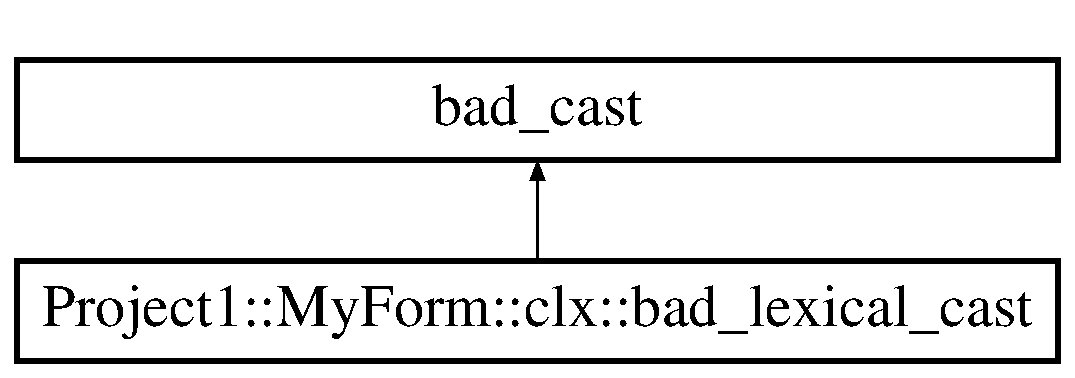
\includegraphics[height=2.000000cm]{class_project1_1_1_my_form_1_1clx_1_1bad__lexical__cast}
\end{center}
\end{figure}
\subsection*{公開メンバ関数}
\begin{DoxyCompactItemize}
\item 
\mbox{\Hypertarget{class_project1_1_1_my_form_1_1clx_1_1bad__lexical__cast_a29c933b0a71e3390a729febcc4359635}\label{class_project1_1_1_my_form_1_1clx_1_1bad__lexical__cast_a29c933b0a71e3390a729febcc4359635}} 
{\bfseries bad\+\_\+lexical\+\_\+cast} (const std\+::type\+\_\+info \&source, const std\+::type\+\_\+info \&target)
\item 
\mbox{\Hypertarget{class_project1_1_1_my_form_1_1clx_1_1bad__lexical__cast_ac753f53410a8a4ed06c21654ce76d5b3}\label{class_project1_1_1_my_form_1_1clx_1_1bad__lexical__cast_ac753f53410a8a4ed06c21654ce76d5b3}} 
const std\+::type\+\_\+info \& {\bfseries source\+\_\+type} () const
\item 
\mbox{\Hypertarget{class_project1_1_1_my_form_1_1clx_1_1bad__lexical__cast_ae0b07193cfe892db01fc8b4fb236d495}\label{class_project1_1_1_my_form_1_1clx_1_1bad__lexical__cast_ae0b07193cfe892db01fc8b4fb236d495}} 
const std\+::type\+\_\+info \& {\bfseries target\+\_\+type} () const
\item 
\mbox{\Hypertarget{class_project1_1_1_my_form_1_1clx_1_1bad__lexical__cast_a0935bb29f2da56fd7e44d398769cef4a}\label{class_project1_1_1_my_form_1_1clx_1_1bad__lexical__cast_a0935bb29f2da56fd7e44d398769cef4a}} 
virtual const char $\ast$ {\bfseries what} () const  throw ()
\end{DoxyCompactItemize}


このクラス詳解は次のファイルから抽出されました\+:\begin{DoxyCompactItemize}
\item 
U\+I/\+Project1/My\+Form.\+h\end{DoxyCompactItemize}

\hypertarget{class_project1_1_1_my_form_1_1clx_1_1cast__stream}{}\section{Project1\+:\+:My\+Form\+:\+:clx\+:\+:cast\+\_\+stream$<$ Type, Source $>$ クラステンプレート}
\label{class_project1_1_1_my_form_1_1clx_1_1cast__stream}\index{Project1\+::\+My\+Form\+::clx\+::cast\+\_\+stream$<$ Type, Source $>$@{Project1\+::\+My\+Form\+::clx\+::cast\+\_\+stream$<$ Type, Source $>$}}
\subsection*{公開型}
\begin{DoxyCompactItemize}
\item 
\mbox{\Hypertarget{class_project1_1_1_my_form_1_1clx_1_1cast__stream_af0a537f7df0557254490387977c545ba}\label{class_project1_1_1_my_form_1_1clx_1_1cast__stream_af0a537f7df0557254490387977c545ba}} 
typedef Source {\bfseries src\+\_\+type}
\item 
\mbox{\Hypertarget{class_project1_1_1_my_form_1_1clx_1_1cast__stream_af58084766d001872f4b3f64ee7c0c300}\label{class_project1_1_1_my_form_1_1clx_1_1cast__stream_af58084766d001872f4b3f64ee7c0c300}} 
typedef Type {\bfseries dest\+\_\+type}
\item 
\mbox{\Hypertarget{class_project1_1_1_my_form_1_1clx_1_1cast__stream_a0bbc71a4347cbdc9cd20b2428ba4e236}\label{class_project1_1_1_my_form_1_1clx_1_1cast__stream_a0bbc71a4347cbdc9cd20b2428ba4e236}} 
typedef \hyperlink{struct_project1_1_1_my_form_1_1clx_1_1detail_1_1widest__char}{detail\+::widest\+\_\+char}$<$ typename \hyperlink{struct_project1_1_1_my_form_1_1clx_1_1detail_1_1stream__char}{detail\+::stream\+\_\+char}$<$ Type $>$\+::type, typename \hyperlink{struct_project1_1_1_my_form_1_1clx_1_1detail_1_1stream__char}{detail\+::stream\+\_\+char}$<$ Source $>$\+::type $>$\+::type {\bfseries char\+\_\+type}
\item 
\mbox{\Hypertarget{class_project1_1_1_my_form_1_1clx_1_1cast__stream_aac4589e719ad0437cfc7951ed6939057}\label{class_project1_1_1_my_form_1_1clx_1_1cast__stream_aac4589e719ad0437cfc7951ed6939057}} 
typedef std\+::basic\+\_\+string$<$ char\+\_\+type $>$ {\bfseries string\+\_\+type}
\item 
\mbox{\Hypertarget{class_project1_1_1_my_form_1_1clx_1_1cast__stream_a6dccdd3ed78cd25dbd6dfef270ab9cf7}\label{class_project1_1_1_my_form_1_1clx_1_1cast__stream_a6dccdd3ed78cd25dbd6dfef270ab9cf7}} 
typedef std\+::basic\+\_\+stringstream$<$ char\+\_\+type $>$ {\bfseries internal\+\_\+stream}
\end{DoxyCompactItemize}
\subsection*{公開メンバ関数}
\begin{DoxyCompactItemize}
\item 
\mbox{\Hypertarget{class_project1_1_1_my_form_1_1clx_1_1cast__stream_a387f08a56ab764c21704f1ee8c21ae86}\label{class_project1_1_1_my_form_1_1clx_1_1cast__stream_a387f08a56ab764c21704f1ee8c21ae86}} 
{\bfseries cast\+\_\+stream} (std\+::ios\+::fmtflags base=std\+::ios\+::dec)
\item 
\mbox{\Hypertarget{class_project1_1_1_my_form_1_1clx_1_1cast__stream_a0c73a6a819948c22efb053af7a7cf54d}\label{class_project1_1_1_my_form_1_1clx_1_1cast__stream_a0c73a6a819948c22efb053af7a7cf54d}} 
bool {\bfseries operator$<$$<$} (const src\+\_\+type \&src)
\item 
\mbox{\Hypertarget{class_project1_1_1_my_form_1_1clx_1_1cast__stream_af016c1601747a5a98aaf73cab36e40e5}\label{class_project1_1_1_my_form_1_1clx_1_1cast__stream_af016c1601747a5a98aaf73cab36e40e5}} 
{\footnotesize template$<$class ValueT $>$ }\\bool {\bfseries operator$>$$>$} (ValueT \&dest)
\item 
\mbox{\Hypertarget{class_project1_1_1_my_form_1_1clx_1_1cast__stream_aaeaf3ceeb2ad1c037fc5f2a8c24f23d3}\label{class_project1_1_1_my_form_1_1clx_1_1cast__stream_aaeaf3ceeb2ad1c037fc5f2a8c24f23d3}} 
bool {\bfseries operator$>$$>$} (string\+\_\+type \&dest)
\end{DoxyCompactItemize}


このクラス詳解は次のファイルから抽出されました\+:\begin{DoxyCompactItemize}
\item 
U\+I/\+Project1/My\+Form.\+h\end{DoxyCompactItemize}

\hypertarget{class_project1_1_1_my_form_1_1clx_1_1charset__functor}{}\section{Project1\+:\+:My\+Form\+:\+:clx\+:\+:charset\+\_\+functor$<$ CharT $>$ クラステンプレート}
\label{class_project1_1_1_my_form_1_1clx_1_1charset__functor}\index{Project1\+::\+My\+Form\+::clx\+::charset\+\_\+functor$<$ Char\+T $>$@{Project1\+::\+My\+Form\+::clx\+::charset\+\_\+functor$<$ Char\+T $>$}}
\subsection*{公開型}
\begin{DoxyCompactItemize}
\item 
\mbox{\Hypertarget{class_project1_1_1_my_form_1_1clx_1_1charset__functor_af46a677fedd21f2dd81e8e2f6d92871e}\label{class_project1_1_1_my_form_1_1clx_1_1charset__functor_af46a677fedd21f2dd81e8e2f6d92871e}} 
typedef CharT {\bfseries char\+\_\+type}
\item 
\mbox{\Hypertarget{class_project1_1_1_my_form_1_1clx_1_1charset__functor_a085c2a025adffe0c9585999580e36d4b}\label{class_project1_1_1_my_form_1_1clx_1_1charset__functor_a085c2a025adffe0c9585999580e36d4b}} 
typedef unsigned int {\bfseries size\+\_\+type}
\end{DoxyCompactItemize}
\subsection*{公開メンバ関数}
\begin{DoxyCompactItemize}
\item 
\mbox{\Hypertarget{class_project1_1_1_my_form_1_1clx_1_1charset__functor_a3520f73cbbd9d52daa0d574804a346a9}\label{class_project1_1_1_my_form_1_1clx_1_1charset__functor_a3520f73cbbd9d52daa0d574804a346a9}} 
{\bfseries charset\+\_\+functor} (const char\+\_\+type $\ast$s)
\item 
\mbox{\Hypertarget{class_project1_1_1_my_form_1_1clx_1_1charset__functor_a4e3d94cad00f37f1240e4b892503f5ad}\label{class_project1_1_1_my_form_1_1clx_1_1charset__functor_a4e3d94cad00f37f1240e4b892503f5ad}} 
{\bfseries charset\+\_\+functor} (const std\+::basic\+\_\+string$<$ CharT $>$ \&s)
\item 
\mbox{\Hypertarget{class_project1_1_1_my_form_1_1clx_1_1charset__functor_afa975ba6f5be1d62a25349ab63324dcb}\label{class_project1_1_1_my_form_1_1clx_1_1charset__functor_afa975ba6f5be1d62a25349ab63324dcb}} 
bool {\bfseries operator()} (char\+\_\+type c) const
\end{DoxyCompactItemize}


このクラス詳解は次のファイルから抽出されました\+:\begin{DoxyCompactItemize}
\item 
U\+I/\+Project1/My\+Form.\+h\end{DoxyCompactItemize}

\hypertarget{class_project1_1_1_my_form_1_1clx_1_1classified__functor}{}\section{Project1\+:\+:My\+Form\+:\+:clx\+:\+:classified\+\_\+functor クラス}
\label{class_project1_1_1_my_form_1_1clx_1_1classified__functor}\index{Project1\+::\+My\+Form\+::clx\+::classified\+\_\+functor@{Project1\+::\+My\+Form\+::clx\+::classified\+\_\+functor}}
\subsection*{公開メンバ関数}
\begin{DoxyCompactItemize}
\item 
\mbox{\Hypertarget{class_project1_1_1_my_form_1_1clx_1_1classified__functor_aa57ebeb1e93b96b0c0fb3f90aa3459d0}\label{class_project1_1_1_my_form_1_1clx_1_1classified__functor_aa57ebeb1e93b96b0c0fb3f90aa3459d0}} 
{\bfseries classified\+\_\+functor} (std\+::ctype\+\_\+base\+::mask m, const std\+::locale \&loc=std\+::locale())
\item 
\mbox{\Hypertarget{class_project1_1_1_my_form_1_1clx_1_1classified__functor_aaf89c98c3bcbe1f6d696d3f229fb8d2b}\label{class_project1_1_1_my_form_1_1clx_1_1classified__functor_aaf89c98c3bcbe1f6d696d3f229fb8d2b}} 
{\footnotesize template$<$class CharT $>$ }\\bool {\bfseries operator()} (CharT c) const
\end{DoxyCompactItemize}


このクラス詳解は次のファイルから抽出されました\+:\begin{DoxyCompactItemize}
\item 
My\+Form.\+h\end{DoxyCompactItemize}

\hypertarget{struct_d_e_v_i_c_e}{}\section{D\+E\+V\+I\+CE 構造体}
\label{struct_d_e_v_i_c_e}\index{D\+E\+V\+I\+CE@{D\+E\+V\+I\+CE}}
\subsection*{公開変数類}
\begin{DoxyCompactItemize}
\item 
\mbox{\Hypertarget{struct_d_e_v_i_c_e_a3437c54a22f99806d6ed2de7ce111942}\label{struct_d_e_v_i_c_e_a3437c54a22f99806d6ed2de7ce111942}} 
int {\bfseries device\+\_\+id}
\item 
\mbox{\Hypertarget{struct_d_e_v_i_c_e_acdc0506b80caaef845d091a70b4863d1}\label{struct_d_e_v_i_c_e_acdc0506b80caaef845d091a70b4863d1}} 
int {\bfseries wire\+\_\+type}
\item 
\mbox{\Hypertarget{struct_d_e_v_i_c_e_a3ff80bbb695010b27b7ced05c8ec04ae}\label{struct_d_e_v_i_c_e_a3ff80bbb695010b27b7ced05c8ec04ae}} 
char {\bfseries adress} \mbox{[}256\mbox{]}
\item 
\mbox{\Hypertarget{struct_d_e_v_i_c_e_ac1c9868f69ed36d904cb2f725e36c18f}\label{struct_d_e_v_i_c_e_ac1c9868f69ed36d904cb2f725e36c18f}} 
char {\bfseries name} \mbox{[}256\mbox{]}
\item 
\mbox{\Hypertarget{struct_d_e_v_i_c_e_adbb1540fbc519029ecd73747c0a24773}\label{struct_d_e_v_i_c_e_adbb1540fbc519029ecd73747c0a24773}} 
char {\bfseries file\+\_\+name\+\_\+header} \mbox{[}32\mbox{]}
\item 
\mbox{\Hypertarget{struct_d_e_v_i_c_e_abbd372951f35b2703c768c260ecb7817}\label{struct_d_e_v_i_c_e_abbd372951f35b2703c768c260ecb7817}} 
char {\bfseries file\+\_\+path} \mbox{[}32\mbox{]}
\end{DoxyCompactItemize}


この構造体詳解は次のファイルから抽出されました\+:\begin{DoxyCompactItemize}
\item 
tkadc.\+h\end{DoxyCompactItemize}

\hypertarget{classexadcstart}{}\section{exadcstart クラス}
\label{classexadcstart}\index{exadcstart@{exadcstart}}
\subsection*{公開メンバ関数}
\begin{DoxyCompactItemize}
\item 
\mbox{\Hypertarget{classexadcstart_aebb1382ce90d77c855319da9087fdf25}\label{classexadcstart_aebb1382ce90d77c855319da9087fdf25}} 
{\bfseries exadcstart} (T\+K\+A\+D\+C\+I\+N\+F\+O\+::\+A\+D\+C\+ID const adcid\+\_\+, \hyperlink{class_t_k_a_d_c_c_o_n_t_r_o_l_a4ec8bb3e68a489f7a757d08a855ffb61}{T\+K\+A\+D\+C\+C\+O\+N\+T\+R\+O\+L\+::\+C\+O\+N\+D\+I\+T\+I\+O\+N\+F\+L\+AG} flag\+\_\+)
\item 
\mbox{\Hypertarget{classexadcstart_aaf643294d3a2081a502affb98baf7d8d}\label{classexadcstart_aaf643294d3a2081a502affb98baf7d8d}} 
void {\bfseries operator()} ()
\end{DoxyCompactItemize}


このクラス詳解は次のファイルから抽出されました\+:\begin{DoxyCompactItemize}
\item 
U\+I/\+Project1/My\+Form.\+h\end{DoxyCompactItemize}

\hypertarget{classexfunctor}{}\section{exfunctor クラス}
\label{classexfunctor}\index{exfunctor@{exfunctor}}
\subsection*{公開メンバ関数}
\begin{DoxyCompactItemize}
\item 
\mbox{\Hypertarget{classexfunctor_a046e03c5618e10bc3a3145af0fe97c6d}\label{classexfunctor_a046e03c5618e10bc3a3145af0fe97c6d}} 
{\bfseries exfunctor} (clx\+::ini $\ast$const Setting\+\_\+, T\+K\+A\+D\+C\+I\+N\+F\+O\+::\+A\+D\+C\+ID const adcid\+\_\+, \hyperlink{class_t_k_a_d_c_c_o_n_t_r_o_l_a4ec8bb3e68a489f7a757d08a855ffb61}{T\+K\+A\+D\+C\+C\+O\+N\+T\+R\+O\+L\+::\+C\+O\+N\+D\+I\+T\+I\+O\+N\+F\+L\+AG} flag\+\_\+)
\item 
\mbox{\Hypertarget{classexfunctor_add31fc15807f9bc3efe7761173213c44}\label{classexfunctor_add31fc15807f9bc3efe7761173213c44}} 
void {\bfseries operator()} ()
\end{DoxyCompactItemize}


このクラス詳解は次のファイルから抽出されました\+:\begin{DoxyCompactItemize}
\item 
U\+I/\+Project1/My\+Form.\+h\end{DoxyCompactItemize}

\hypertarget{class_project1_1_1_my_form}{}\section{Project1\+:\+:My\+Form クラス}
\label{class_project1_1_1_my_form}\index{Project1\+::\+My\+Form@{Project1\+::\+My\+Form}}


\hyperlink{class_project1_1_1_my_form}{My\+Form} の概要  




{\ttfamily \#include $<$My\+Form.\+h$>$}

Project1\+:\+:My\+Form の継承関係図\begin{figure}[H]
\begin{center}
\leavevmode
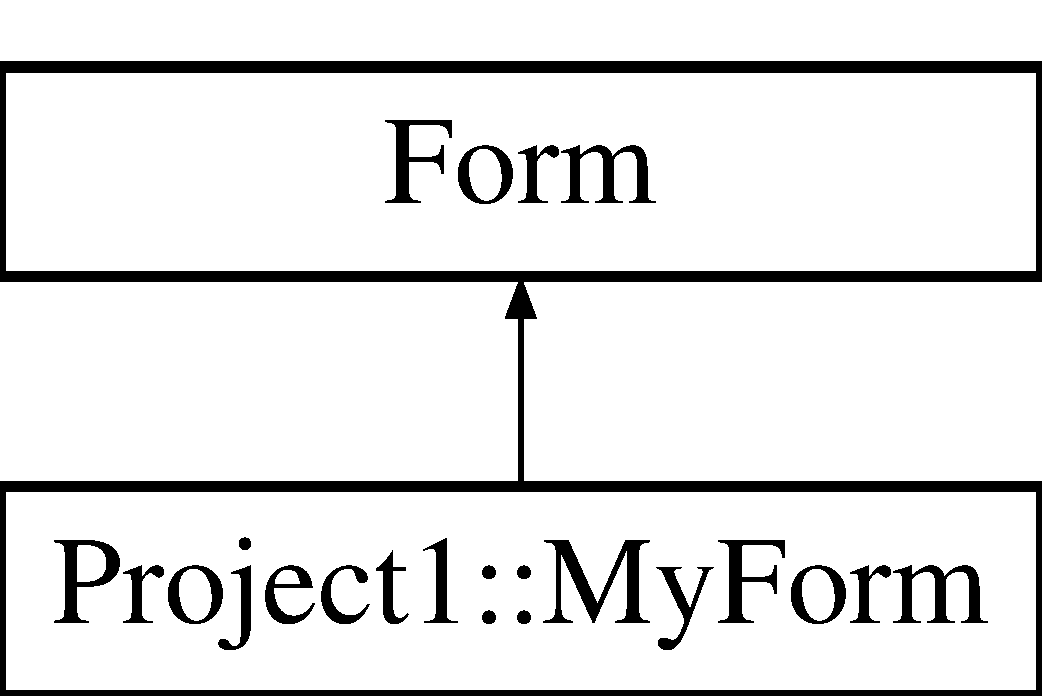
\includegraphics[height=2.000000cm]{class_project1_1_1_my_form}
\end{center}
\end{figure}
\subsection*{公開メンバ関数}
\begin{DoxyCompactItemize}
\item 
\mbox{\Hypertarget{class_project1_1_1_my_form_a2d96004e6380e1bdfffe4675083b6769}\label{class_project1_1_1_my_form_a2d96004e6380e1bdfffe4675083b6769}} 
{\bfseries My\+Form} (clx\+::ini $\ast$Setting\+\_\+, \hyperlink{class_t_k_s_h_o_t}{T\+K\+S\+H\+OT} $\ast$this\+Shot\+\_\+, \hyperlink{class_t_k_p_l_o_t}{T\+K\+P\+L\+OT} $\ast$this\+Plot\+\_\+, \hyperlink{class_t_k_a_d_c_c_o_n_t_r_o_l___d_l750}{T\+K\+A\+D\+C\+C\+O\+N\+T\+R\+O\+L\+\_\+\+D\+L750} $\ast$D\+L750\+\_\+, \hyperlink{class_t_k_a_d_c_c_o_n_t_r_o_l___d_l850}{T\+K\+A\+D\+C\+C\+O\+N\+T\+R\+O\+L\+\_\+\+D\+L850} $\ast$D\+L850\+\_\+)
\end{DoxyCompactItemize}
\subsection*{限定公開メンバ関数}
\begin{DoxyCompactItemize}
\item 
\hyperlink{class_project1_1_1_my_form_a501b2b4481b72877fc73101f1d6f26be}{$\sim$\+My\+Form} ()
\begin{DoxyCompactList}\small\item\em 使用中のリソースをすべてクリーンアップします。 \end{DoxyCompactList}\end{DoxyCompactItemize}


\subsection{詳解}
\hyperlink{class_project1_1_1_my_form}{My\+Form} の概要 



\subsection{構築子と解体子}
\mbox{\Hypertarget{class_project1_1_1_my_form_a501b2b4481b72877fc73101f1d6f26be}\label{class_project1_1_1_my_form_a501b2b4481b72877fc73101f1d6f26be}} 
\index{Project1\+::\+My\+Form@{Project1\+::\+My\+Form}!````~My\+Form@{$\sim$\+My\+Form}}
\index{````~My\+Form@{$\sim$\+My\+Form}!Project1\+::\+My\+Form@{Project1\+::\+My\+Form}}
\subsubsection{\texorpdfstring{$\sim$\+My\+Form()}{~MyForm()}}
{\footnotesize\ttfamily Project1\+::\+My\+Form\+::$\sim$\+My\+Form (\begin{DoxyParamCaption}{ }\end{DoxyParamCaption})\hspace{0.3cm}{\ttfamily [inline]}, {\ttfamily [protected]}}



使用中のリソースをすべてクリーンアップします。 



このクラス詳解は次のファイルから抽出されました\+:\begin{DoxyCompactItemize}
\item 
U\+I/\+Project1/My\+Form.\+h\item 
U\+I/\+Project1/My\+Form.\+cpp\end{DoxyCompactItemize}

\hypertarget{struct_t_k_p_l_o_t_1_1_p_l_o_t_i_n_f_o}{}\section{T\+K\+P\+L\+OT\+:\+:P\+L\+O\+T\+I\+N\+FO 構造体}
\label{struct_t_k_p_l_o_t_1_1_p_l_o_t_i_n_f_o}\index{T\+K\+P\+L\+O\+T\+::\+P\+L\+O\+T\+I\+N\+FO@{T\+K\+P\+L\+O\+T\+::\+P\+L\+O\+T\+I\+N\+FO}}
\subsection*{公開変数類}
\begin{DoxyCompactItemize}
\item 
\mbox{\Hypertarget{struct_t_k_p_l_o_t_1_1_p_l_o_t_i_n_f_o_ac1dae6b6cd429f4276f5a4491af8c24d}\label{struct_t_k_p_l_o_t_1_1_p_l_o_t_i_n_f_o_ac1dae6b6cd429f4276f5a4491af8c24d}} 
std\+::string {\bfseries plot\+\_\+file\+\_\+name}
\item 
\mbox{\Hypertarget{struct_t_k_p_l_o_t_1_1_p_l_o_t_i_n_f_o_a18a67313f8bb54564f35f6e6eddef899}\label{struct_t_k_p_l_o_t_1_1_p_l_o_t_i_n_f_o_a18a67313f8bb54564f35f6e6eddef899}} 
std\+::string {\bfseries data\+\_\+file\+\_\+name}
\item 
\mbox{\Hypertarget{struct_t_k_p_l_o_t_1_1_p_l_o_t_i_n_f_o_a48ef8281322bf15a1e48cca923d34eeb}\label{struct_t_k_p_l_o_t_1_1_p_l_o_t_i_n_f_o_a48ef8281322bf15a1e48cca923d34eeb}} 
int {\bfseries trace\+\_\+index}
\item 
\mbox{\Hypertarget{struct_t_k_p_l_o_t_1_1_p_l_o_t_i_n_f_o_a13b0235f3544b9d875af92ce3ac247ab}\label{struct_t_k_p_l_o_t_1_1_p_l_o_t_i_n_f_o_a13b0235f3544b9d875af92ce3ac247ab}} 
\hyperlink{class_t_k_p_l_o_t_1_1_r_a_n_g_e}{T\+K\+P\+L\+O\+T\+::\+R\+A\+N\+GE}$<$ float $>$ {\bfseries xrange}
\item 
\mbox{\Hypertarget{struct_t_k_p_l_o_t_1_1_p_l_o_t_i_n_f_o_a5ce7809252eb582e3fae0a554bcdb65d}\label{struct_t_k_p_l_o_t_1_1_p_l_o_t_i_n_f_o_a5ce7809252eb582e3fae0a554bcdb65d}} 
\hyperlink{class_t_k_p_l_o_t_1_1_r_a_n_g_e}{T\+K\+P\+L\+O\+T\+::\+R\+A\+N\+GE}$<$ float $>$ {\bfseries yrange}
\item 
\mbox{\Hypertarget{struct_t_k_p_l_o_t_1_1_p_l_o_t_i_n_f_o_ab210e72c1f8d1e3d930b003f47568d3e}\label{struct_t_k_p_l_o_t_1_1_p_l_o_t_i_n_f_o_ab210e72c1f8d1e3d930b003f47568d3e}} 
int {\bfseries every}
\item 
\mbox{\Hypertarget{struct_t_k_p_l_o_t_1_1_p_l_o_t_i_n_f_o_ae98bf84fdf14074b4f7804f0617aa902}\label{struct_t_k_p_l_o_t_1_1_p_l_o_t_i_n_f_o_ae98bf84fdf14074b4f7804f0617aa902}} 
std\+::string {\bfseries model\+\_\+name}
\item 
\mbox{\Hypertarget{struct_t_k_p_l_o_t_1_1_p_l_o_t_i_n_f_o_a801d16eb357241d4f4eeef8c6393bbc4}\label{struct_t_k_p_l_o_t_1_1_p_l_o_t_i_n_f_o_a801d16eb357241d4f4eeef8c6393bbc4}} 
int {\bfseries channel\+\_\+number}
\item 
\mbox{\Hypertarget{struct_t_k_p_l_o_t_1_1_p_l_o_t_i_n_f_o_a8e6f18f0fb90610f38ca893614565c58}\label{struct_t_k_p_l_o_t_1_1_p_l_o_t_i_n_f_o_a8e6f18f0fb90610f38ca893614565c58}} 
float {\bfseries h\+\_\+resolution}
\item 
\mbox{\Hypertarget{struct_t_k_p_l_o_t_1_1_p_l_o_t_i_n_f_o_afe6df040b952e6ab1e234d17de6023d0}\label{struct_t_k_p_l_o_t_1_1_p_l_o_t_i_n_f_o_afe6df040b952e6ab1e234d17de6023d0}} 
\hyperlink{class_t_k_p_l_o_t_1_1_s_i_z_e}{S\+I\+ZE}$<$ int $>$ {\bfseries terminal\+\_\+size}
\item 
\mbox{\Hypertarget{struct_t_k_p_l_o_t_1_1_p_l_o_t_i_n_f_o_a27451bd9ddcd548bff9f91cdda6ed812}\label{struct_t_k_p_l_o_t_1_1_p_l_o_t_i_n_f_o_a27451bd9ddcd548bff9f91cdda6ed812}} 
\hyperlink{class_t_k_p_l_o_t_1_1_s_i_z_e}{S\+I\+ZE}$<$ int $>$ {\bfseries drawing\+\_\+size}
\item 
\mbox{\Hypertarget{struct_t_k_p_l_o_t_1_1_p_l_o_t_i_n_f_o_ad5e1f688a044784cf24846d04fd48116}\label{struct_t_k_p_l_o_t_1_1_p_l_o_t_i_n_f_o_ad5e1f688a044784cf24846d04fd48116}} 
\hyperlink{class_t_k_p_l_o_t_1_1_p_o_s_i_t_i_o_n}{P\+O\+S\+I\+T\+I\+ON}$<$ int $>$ {\bfseries drawing\+\_\+origin}
\item 
\mbox{\Hypertarget{struct_t_k_p_l_o_t_1_1_p_l_o_t_i_n_f_o_a4266fd64b26c45e727843dc017ba2a3d}\label{struct_t_k_p_l_o_t_1_1_p_l_o_t_i_n_f_o_a4266fd64b26c45e727843dc017ba2a3d}} 
std\+::vector$<$ \hyperlink{class_t_k_p_l_o_t_1_1_p_o_s_i_t_i_o_n}{P\+O\+S\+I\+T\+I\+ON}$<$ float $>$ $>$ {\bfseries label\+\_\+position}
\end{DoxyCompactItemize}


この構造体詳解は次のファイルから抽出されました\+:\begin{DoxyCompactItemize}
\item 
tkplot.\+h\end{DoxyCompactItemize}

\hypertarget{class_t_k_p_l_o_t_1_1_p_o_s_i_t_i_o_n}{}\section{T\+K\+P\+L\+OT\+:\+:P\+O\+S\+I\+T\+I\+ON$<$ T $>$ クラステンプレート}
\label{class_t_k_p_l_o_t_1_1_p_o_s_i_t_i_o_n}\index{T\+K\+P\+L\+O\+T\+::\+P\+O\+S\+I\+T\+I\+O\+N$<$ T $>$@{T\+K\+P\+L\+O\+T\+::\+P\+O\+S\+I\+T\+I\+O\+N$<$ T $>$}}
\subsection*{公開メンバ関数}
\begin{DoxyCompactItemize}
\item 
\mbox{\Hypertarget{class_t_k_p_l_o_t_1_1_p_o_s_i_t_i_o_n_abce2e3b6b659c15133abef1c6e35fe1c}\label{class_t_k_p_l_o_t_1_1_p_o_s_i_t_i_o_n_abce2e3b6b659c15133abef1c6e35fe1c}} 
{\bfseries P\+O\+S\+I\+T\+I\+ON} (T x\+\_\+, T y\+\_\+)
\item 
\mbox{\Hypertarget{class_t_k_p_l_o_t_1_1_p_o_s_i_t_i_o_n_a715ead8ec7884aaca1ec220e77c83b03}\label{class_t_k_p_l_o_t_1_1_p_o_s_i_t_i_o_n_a715ead8ec7884aaca1ec220e77c83b03}} 
std\+::string {\bfseries str} ()
\end{DoxyCompactItemize}
\subsection*{公開変数類}
\begin{DoxyCompactItemize}
\item 
\mbox{\Hypertarget{class_t_k_p_l_o_t_1_1_p_o_s_i_t_i_o_n_a260fc49a5e31e7dd5d42fc01b05a88f7}\label{class_t_k_p_l_o_t_1_1_p_o_s_i_t_i_o_n_a260fc49a5e31e7dd5d42fc01b05a88f7}} 
T {\bfseries x}
\item 
\mbox{\Hypertarget{class_t_k_p_l_o_t_1_1_p_o_s_i_t_i_o_n_ae84c7221f133098571c5389d76285591}\label{class_t_k_p_l_o_t_1_1_p_o_s_i_t_i_o_n_ae84c7221f133098571c5389d76285591}} 
T {\bfseries y}
\item 
\mbox{\Hypertarget{class_t_k_p_l_o_t_1_1_p_o_s_i_t_i_o_n_a023ad2c7a8239540613a5b18c70772ff}\label{class_t_k_p_l_o_t_1_1_p_o_s_i_t_i_o_n_a023ad2c7a8239540613a5b18c70772ff}} 
T \& {\bfseries u} = x
\item 
\mbox{\Hypertarget{class_t_k_p_l_o_t_1_1_p_o_s_i_t_i_o_n_a776d51b19318a7177128c435eae80a48}\label{class_t_k_p_l_o_t_1_1_p_o_s_i_t_i_o_n_a776d51b19318a7177128c435eae80a48}} 
T \& {\bfseries v} = y
\end{DoxyCompactItemize}


このクラス詳解は次のファイルから抽出されました\+:\begin{DoxyCompactItemize}
\item 
tkplot.\+h\end{DoxyCompactItemize}

\hypertarget{class_t_k_p_l_o_t_1_1_r_a_n_g_e}{}\section{T\+K\+P\+L\+OT\+:\+:R\+A\+N\+GE$<$ T $>$ クラステンプレート}
\label{class_t_k_p_l_o_t_1_1_r_a_n_g_e}\index{T\+K\+P\+L\+O\+T\+::\+R\+A\+N\+G\+E$<$ T $>$@{T\+K\+P\+L\+O\+T\+::\+R\+A\+N\+G\+E$<$ T $>$}}
\subsection*{公開メンバ関数}
\begin{DoxyCompactItemize}
\item 
\mbox{\Hypertarget{class_t_k_p_l_o_t_1_1_r_a_n_g_e_a15cccdb1c926b077c9f06173a5d144a5}\label{class_t_k_p_l_o_t_1_1_r_a_n_g_e_a15cccdb1c926b077c9f06173a5d144a5}} 
{\bfseries R\+A\+N\+GE} (T min\+\_\+, T max\+\_\+)
\item 
\mbox{\Hypertarget{class_t_k_p_l_o_t_1_1_r_a_n_g_e_aada3563138773d6575a67eed99dc8c1b}\label{class_t_k_p_l_o_t_1_1_r_a_n_g_e_aada3563138773d6575a67eed99dc8c1b}} 
std\+::string {\bfseries str} ()
\item 
\mbox{\Hypertarget{class_t_k_p_l_o_t_1_1_r_a_n_g_e_ace282f2a0952d3cca69702556ef92836}\label{class_t_k_p_l_o_t_1_1_r_a_n_g_e_ace282f2a0952d3cca69702556ef92836}} 
T {\bfseries median} ()
\end{DoxyCompactItemize}
\subsection*{公開変数類}
\begin{DoxyCompactItemize}
\item 
\mbox{\Hypertarget{class_t_k_p_l_o_t_1_1_r_a_n_g_e_af83dec2420b2e2d8629d212475a49fee}\label{class_t_k_p_l_o_t_1_1_r_a_n_g_e_af83dec2420b2e2d8629d212475a49fee}} 
T {\bfseries min}
\item 
\mbox{\Hypertarget{class_t_k_p_l_o_t_1_1_r_a_n_g_e_a7100fa300f2cffeed4e5f0657afea787}\label{class_t_k_p_l_o_t_1_1_r_a_n_g_e_a7100fa300f2cffeed4e5f0657afea787}} 
T {\bfseries max}
\end{DoxyCompactItemize}


このクラス詳解は次のファイルから抽出されました\+:\begin{DoxyCompactItemize}
\item 
U\+I/\+Project1/tkplot.\+h\end{DoxyCompactItemize}

\hypertarget{class_project1_1_1_setup_a_d_c_connection}{}\section{Project1\+:\+:Setup\+A\+D\+C\+Connection クラス}
\label{class_project1_1_1_setup_a_d_c_connection}\index{Project1\+::\+Setup\+A\+D\+C\+Connection@{Project1\+::\+Setup\+A\+D\+C\+Connection}}


\hyperlink{class_project1_1_1_setup_a_d_c_connection}{Setup\+A\+D\+C\+Connection} �̊\+T�v  




{\ttfamily \#include $<$Setup\+A\+D\+C\+Connection.\+h$>$}

Project1\+:\+:Setup\+A\+D\+C\+Connection の継承関係図\begin{figure}[H]
\begin{center}
\leavevmode
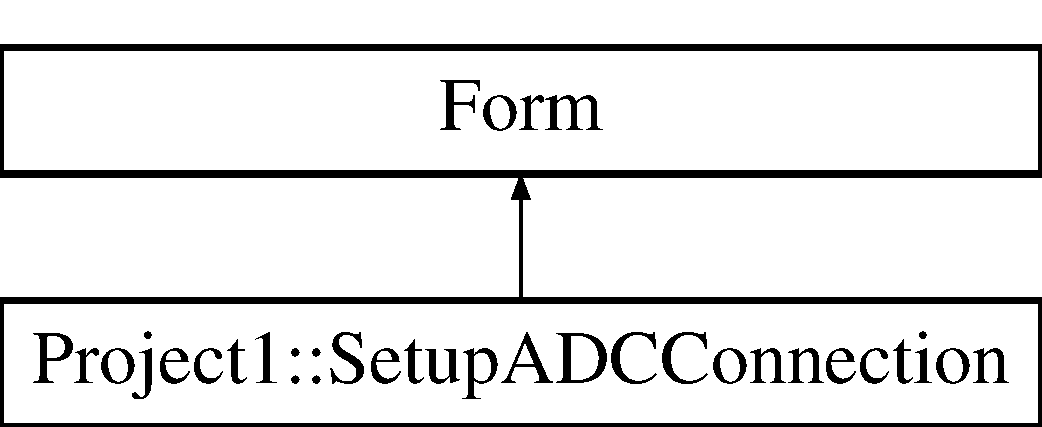
\includegraphics[height=2.000000cm]{class_project1_1_1_setup_a_d_c_connection}
\end{center}
\end{figure}
\subsection*{公開メンバ関数}
\begin{DoxyCompactItemize}
\item 
\mbox{\Hypertarget{class_project1_1_1_setup_a_d_c_connection_ace927052e2be7c56f451eb04559d34d6}\label{class_project1_1_1_setup_a_d_c_connection_ace927052e2be7c56f451eb04559d34d6}} 
{\bfseries Setup\+A\+D\+C\+Connection} (clx\+::ini $\ast$Setting\+\_\+)
\end{DoxyCompactItemize}
\subsection*{限定公開メンバ関数}
\begin{DoxyCompactItemize}
\item 
\hyperlink{class_project1_1_1_setup_a_d_c_connection_a866e7e75c329629e9f2d18ff382a7dc4}{$\sim$\+Setup\+A\+D\+C\+Connection} ()
\begin{DoxyCompactList}\small\item\em �g�p���̃��\textbackslash{}�\mbox{[}�\+X�����ׂă\+N���\mbox{[}���\+A�b�v���܂��B \end{DoxyCompactList}\end{DoxyCompactItemize}


\subsection{詳解}
\hyperlink{class_project1_1_1_setup_a_d_c_connection}{Setup\+A\+D\+C\+Connection} �̊\+T�v 



\subsection{構築子と解体子}
\mbox{\Hypertarget{class_project1_1_1_setup_a_d_c_connection_a866e7e75c329629e9f2d18ff382a7dc4}\label{class_project1_1_1_setup_a_d_c_connection_a866e7e75c329629e9f2d18ff382a7dc4}} 
\index{Project1\+::\+Setup\+A\+D\+C\+Connection@{Project1\+::\+Setup\+A\+D\+C\+Connection}!````~Setup\+A\+D\+C\+Connection@{$\sim$\+Setup\+A\+D\+C\+Connection}}
\index{````~Setup\+A\+D\+C\+Connection@{$\sim$\+Setup\+A\+D\+C\+Connection}!Project1\+::\+Setup\+A\+D\+C\+Connection@{Project1\+::\+Setup\+A\+D\+C\+Connection}}
\subsubsection{\texorpdfstring{$\sim$\+Setup\+A\+D\+C\+Connection()}{~SetupADCConnection()}}
{\footnotesize\ttfamily Project1\+::\+Setup\+A\+D\+C\+Connection\+::$\sim$\+Setup\+A\+D\+C\+Connection (\begin{DoxyParamCaption}{ }\end{DoxyParamCaption})\hspace{0.3cm}{\ttfamily [inline]}, {\ttfamily [protected]}}



�g�p���̃��\textbackslash{}�\mbox{[}�\+X�����ׂă\+N���\mbox{[}���\+A�b�v���܂��B 



このクラス詳解は次のファイルから抽出されました\+:\begin{DoxyCompactItemize}
\item 
Setup\+A\+D\+C\+Connection.\+h\end{DoxyCompactItemize}

\hypertarget{class_project1_1_1_setup_a_d_c_measurement}{}\section{Project1\+:\+:Setup\+A\+D\+C\+Measurement クラス}
\label{class_project1_1_1_setup_a_d_c_measurement}\index{Project1\+::\+Setup\+A\+D\+C\+Measurement@{Project1\+::\+Setup\+A\+D\+C\+Measurement}}


\hyperlink{class_project1_1_1_setup_a_d_c_measurement}{Setup\+A\+D\+C\+Measurement} の概要  




{\ttfamily \#include $<$Setup\+A\+D\+C\+Measurement.\+h$>$}

Project1\+:\+:Setup\+A\+D\+C\+Measurement の継承関係図\begin{figure}[H]
\begin{center}
\leavevmode
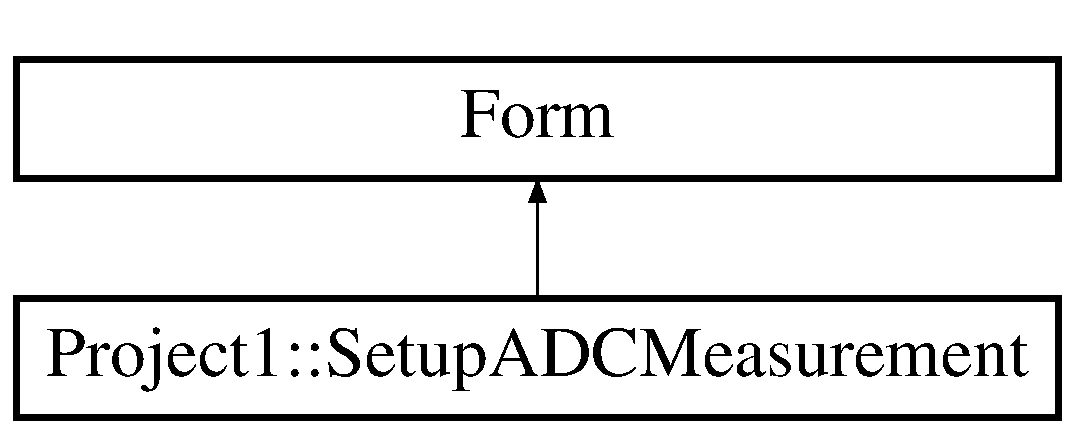
\includegraphics[height=2.000000cm]{class_project1_1_1_setup_a_d_c_measurement}
\end{center}
\end{figure}
\subsection*{限定公開メンバ関数}
\begin{DoxyCompactItemize}
\item 
\hyperlink{class_project1_1_1_setup_a_d_c_measurement_a63b1935cc1f23fc96d175fdb9f1f2fd3}{$\sim$\+Setup\+A\+D\+C\+Measurement} ()
\begin{DoxyCompactList}\small\item\em 使用中のリソースをすべてクリーンアップします。 \end{DoxyCompactList}\end{DoxyCompactItemize}


\subsection{詳解}
\hyperlink{class_project1_1_1_setup_a_d_c_measurement}{Setup\+A\+D\+C\+Measurement} の概要 



\subsection{構築子と解体子}
\mbox{\Hypertarget{class_project1_1_1_setup_a_d_c_measurement_a63b1935cc1f23fc96d175fdb9f1f2fd3}\label{class_project1_1_1_setup_a_d_c_measurement_a63b1935cc1f23fc96d175fdb9f1f2fd3}} 
\index{Project1\+::\+Setup\+A\+D\+C\+Measurement@{Project1\+::\+Setup\+A\+D\+C\+Measurement}!````~Setup\+A\+D\+C\+Measurement@{$\sim$\+Setup\+A\+D\+C\+Measurement}}
\index{````~Setup\+A\+D\+C\+Measurement@{$\sim$\+Setup\+A\+D\+C\+Measurement}!Project1\+::\+Setup\+A\+D\+C\+Measurement@{Project1\+::\+Setup\+A\+D\+C\+Measurement}}
\subsubsection{\texorpdfstring{$\sim$\+Setup\+A\+D\+C\+Measurement()}{~SetupADCMeasurement()}}
{\footnotesize\ttfamily Project1\+::\+Setup\+A\+D\+C\+Measurement\+::$\sim$\+Setup\+A\+D\+C\+Measurement (\begin{DoxyParamCaption}{ }\end{DoxyParamCaption})\hspace{0.3cm}{\ttfamily [inline]}, {\ttfamily [protected]}}



使用中のリソースをすべてクリーンアップします。 



このクラス詳解は次のファイルから抽出されました\+:\begin{DoxyCompactItemize}
\item 
Setup\+A\+D\+C\+Measurement.\+h\end{DoxyCompactItemize}

\hypertarget{class_project1_1_1_setup_analyze_s_p}{}\section{Project1\+:\+:Setup\+Analyze\+SP クラス}
\label{class_project1_1_1_setup_analyze_s_p}\index{Project1\+::\+Setup\+Analyze\+SP@{Project1\+::\+Setup\+Analyze\+SP}}


\hyperlink{class_project1_1_1_setup_analyze_s_p}{Setup\+Analyze\+SP} の概要  




{\ttfamily \#include $<$Setup\+Analyze\+S\+P.\+h$>$}

Project1\+:\+:Setup\+Analyze\+SP の継承関係図\begin{figure}[H]
\begin{center}
\leavevmode
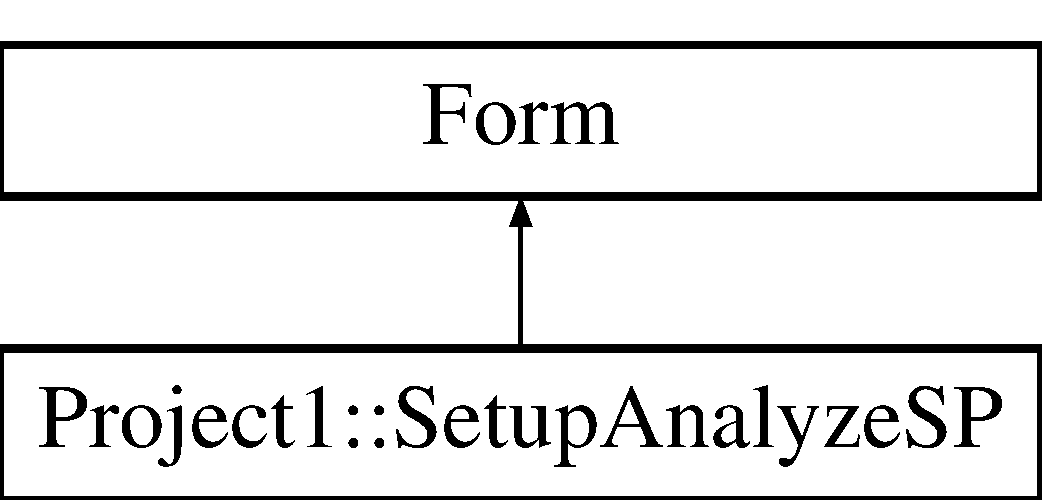
\includegraphics[height=2.000000cm]{class_project1_1_1_setup_analyze_s_p}
\end{center}
\end{figure}
\subsection*{公開メンバ関数}
\begin{DoxyCompactItemize}
\item 
\mbox{\Hypertarget{class_project1_1_1_setup_analyze_s_p_a58fbf31604206da76cead585e94498f2}\label{class_project1_1_1_setup_analyze_s_p_a58fbf31604206da76cead585e94498f2}} 
{\bfseries Setup\+Analyze\+SP} (clx\+::ini $\ast$Setting\+\_\+, \hyperlink{class_t_k_s_h_o_t}{T\+K\+S\+H\+OT} $\ast$this\+Shot\+\_\+, std\+::string group\+\_\+)
\end{DoxyCompactItemize}
\subsection*{限定公開メンバ関数}
\begin{DoxyCompactItemize}
\item 
\hyperlink{class_project1_1_1_setup_analyze_s_p_abb81aeae2341ceec276805a830e94b67}{$\sim$\+Setup\+Analyze\+SP} ()
\begin{DoxyCompactList}\small\item\em 使用中のリソースをすべてクリーンアップします。 \end{DoxyCompactList}\end{DoxyCompactItemize}


\subsection{詳解}
\hyperlink{class_project1_1_1_setup_analyze_s_p}{Setup\+Analyze\+SP} の概要 



\subsection{構築子と解体子}
\mbox{\Hypertarget{class_project1_1_1_setup_analyze_s_p_abb81aeae2341ceec276805a830e94b67}\label{class_project1_1_1_setup_analyze_s_p_abb81aeae2341ceec276805a830e94b67}} 
\index{Project1\+::\+Setup\+Analyze\+SP@{Project1\+::\+Setup\+Analyze\+SP}!````~Setup\+Analyze\+SP@{$\sim$\+Setup\+Analyze\+SP}}
\index{````~Setup\+Analyze\+SP@{$\sim$\+Setup\+Analyze\+SP}!Project1\+::\+Setup\+Analyze\+SP@{Project1\+::\+Setup\+Analyze\+SP}}
\subsubsection{\texorpdfstring{$\sim$\+Setup\+Analyze\+S\+P()}{~SetupAnalyzeSP()}}
{\footnotesize\ttfamily Project1\+::\+Setup\+Analyze\+S\+P\+::$\sim$\+Setup\+Analyze\+SP (\begin{DoxyParamCaption}{ }\end{DoxyParamCaption})\hspace{0.3cm}{\ttfamily [inline]}, {\ttfamily [protected]}}



使用中のリソースをすべてクリーンアップします。 



このクラス詳解は次のファイルから抽出されました\+:\begin{DoxyCompactItemize}
\item 
Setup\+Analyze\+S\+P.\+h\end{DoxyCompactItemize}

\hypertarget{class_project1_1_1_setup_plot}{}\section{Project1\+:\+:Setup\+Plot クラス}
\label{class_project1_1_1_setup_plot}\index{Project1\+::\+Setup\+Plot@{Project1\+::\+Setup\+Plot}}


\hyperlink{class_project1_1_1_setup_plot}{Setup\+Plot} の概要  




{\ttfamily \#include $<$Setup\+Plot.\+h$>$}

Project1\+:\+:Setup\+Plot の継承関係図\begin{figure}[H]
\begin{center}
\leavevmode
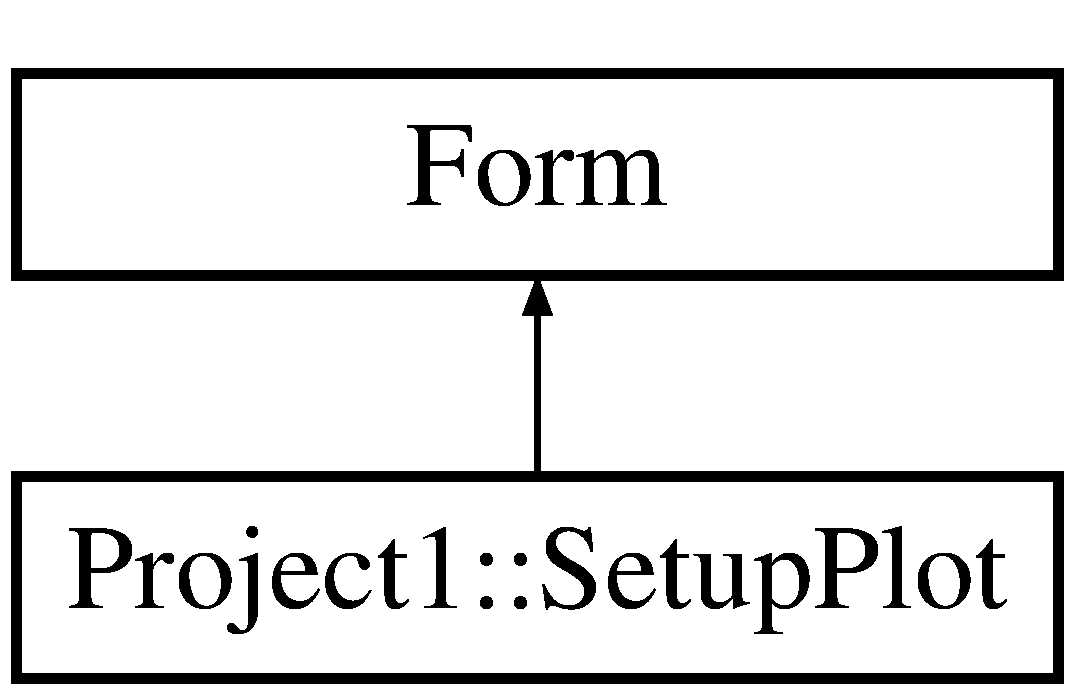
\includegraphics[height=2.000000cm]{class_project1_1_1_setup_plot}
\end{center}
\end{figure}
\subsection*{公開メンバ関数}
\begin{DoxyCompactItemize}
\item 
\mbox{\Hypertarget{class_project1_1_1_setup_plot_a45203c01dce8ca7a6871ff50c10051cd}\label{class_project1_1_1_setup_plot_a45203c01dce8ca7a6871ff50c10051cd}} 
{\bfseries Setup\+Plot} (clx\+::ini $\ast$Shot\+Setting\+\_\+)
\end{DoxyCompactItemize}
\subsection*{限定公開メンバ関数}
\begin{DoxyCompactItemize}
\item 
\hyperlink{class_project1_1_1_setup_plot_a99164cdf31bea63c1f4e01204e381538}{$\sim$\+Setup\+Plot} ()
\begin{DoxyCompactList}\small\item\em 使用中のリソースをすべてクリーンアップします。 \end{DoxyCompactList}\end{DoxyCompactItemize}


\subsection{詳解}
\hyperlink{class_project1_1_1_setup_plot}{Setup\+Plot} の概要 



\subsection{構築子と解体子}
\mbox{\Hypertarget{class_project1_1_1_setup_plot_a99164cdf31bea63c1f4e01204e381538}\label{class_project1_1_1_setup_plot_a99164cdf31bea63c1f4e01204e381538}} 
\index{Project1\+::\+Setup\+Plot@{Project1\+::\+Setup\+Plot}!````~Setup\+Plot@{$\sim$\+Setup\+Plot}}
\index{````~Setup\+Plot@{$\sim$\+Setup\+Plot}!Project1\+::\+Setup\+Plot@{Project1\+::\+Setup\+Plot}}
\subsubsection{\texorpdfstring{$\sim$\+Setup\+Plot()}{~SetupPlot()}}
{\footnotesize\ttfamily Project1\+::\+Setup\+Plot\+::$\sim$\+Setup\+Plot (\begin{DoxyParamCaption}{ }\end{DoxyParamCaption})\hspace{0.3cm}{\ttfamily [inline]}, {\ttfamily [protected]}}



使用中のリソースをすべてクリーンアップします。 



このクラス詳解は次のファイルから抽出されました\+:\begin{DoxyCompactItemize}
\item 
U\+I/\+Project1/Setup\+Plot.\+h\end{DoxyCompactItemize}

\hypertarget{class_t_k_p_l_o_t_1_1_s_i_z_e}{}\section{T\+K\+P\+L\+OT\+:\+:S\+I\+ZE$<$ T $>$ クラステンプレート}
\label{class_t_k_p_l_o_t_1_1_s_i_z_e}\index{T\+K\+P\+L\+O\+T\+::\+S\+I\+Z\+E$<$ T $>$@{T\+K\+P\+L\+O\+T\+::\+S\+I\+Z\+E$<$ T $>$}}
\subsection*{公開メンバ関数}
\begin{DoxyCompactItemize}
\item 
\mbox{\Hypertarget{class_t_k_p_l_o_t_1_1_s_i_z_e_a876e32d89a46cb96f9020c699b43b9ed}\label{class_t_k_p_l_o_t_1_1_s_i_z_e_a876e32d89a46cb96f9020c699b43b9ed}} 
std\+::string {\bfseries str} ()
\end{DoxyCompactItemize}
\subsection*{公開変数類}
\begin{DoxyCompactItemize}
\item 
\mbox{\Hypertarget{class_t_k_p_l_o_t_1_1_s_i_z_e_a11e6a0ae01e934f1f03cd091a778a4f7}\label{class_t_k_p_l_o_t_1_1_s_i_z_e_a11e6a0ae01e934f1f03cd091a778a4f7}} 
T {\bfseries w}
\item 
\mbox{\Hypertarget{class_t_k_p_l_o_t_1_1_s_i_z_e_af53c6cc5ae8485c0e5842ce59783d39e}\label{class_t_k_p_l_o_t_1_1_s_i_z_e_af53c6cc5ae8485c0e5842ce59783d39e}} 
T {\bfseries h}
\item 
\mbox{\Hypertarget{class_t_k_p_l_o_t_1_1_s_i_z_e_ad01852541685a33ee9ac7fb1fbee13bf}\label{class_t_k_p_l_o_t_1_1_s_i_z_e_ad01852541685a33ee9ac7fb1fbee13bf}} 
T \& {\bfseries u} = w
\item 
\mbox{\Hypertarget{class_t_k_p_l_o_t_1_1_s_i_z_e_ac1fb3da1cbaf26656371b68b1f2955a3}\label{class_t_k_p_l_o_t_1_1_s_i_z_e_ac1fb3da1cbaf26656371b68b1f2955a3}} 
T \& {\bfseries v} = h
\end{DoxyCompactItemize}


このクラス詳解は次のファイルから抽出されました\+:\begin{DoxyCompactItemize}
\item 
U\+I/\+Project1/tkplot.\+h\end{DoxyCompactItemize}

\hypertarget{struct_project1_1_1_my_form_1_1clx_1_1detail_1_1stream__char}{}\section{Project1\+:\+:My\+Form\+:\+:clx\+:\+:detail\+:\+:stream\+\_\+char$<$ Type $>$ 構造体テンプレート}
\label{struct_project1_1_1_my_form_1_1clx_1_1detail_1_1stream__char}\index{Project1\+::\+My\+Form\+::clx\+::detail\+::stream\+\_\+char$<$ Type $>$@{Project1\+::\+My\+Form\+::clx\+::detail\+::stream\+\_\+char$<$ Type $>$}}
\subsection*{公開型}
\begin{DoxyCompactItemize}
\item 
\mbox{\Hypertarget{struct_project1_1_1_my_form_1_1clx_1_1detail_1_1stream__char_af3162ed23258265b5a5a3257fd258d55}\label{struct_project1_1_1_my_form_1_1clx_1_1detail_1_1stream__char_af3162ed23258265b5a5a3257fd258d55}} 
typedef char {\bfseries type}
\end{DoxyCompactItemize}


この構造体詳解は次のファイルから抽出されました\+:\begin{DoxyCompactItemize}
\item 
My\+Form.\+h\end{DoxyCompactItemize}

\hypertarget{class_t_k_a_d_c}{}\section{T\+K\+A\+DC クラス}
\label{class_t_k_a_d_c}\index{T\+K\+A\+DC@{T\+K\+A\+DC}}
T\+K\+A\+DC の継承関係図\begin{figure}[H]
\begin{center}
\leavevmode
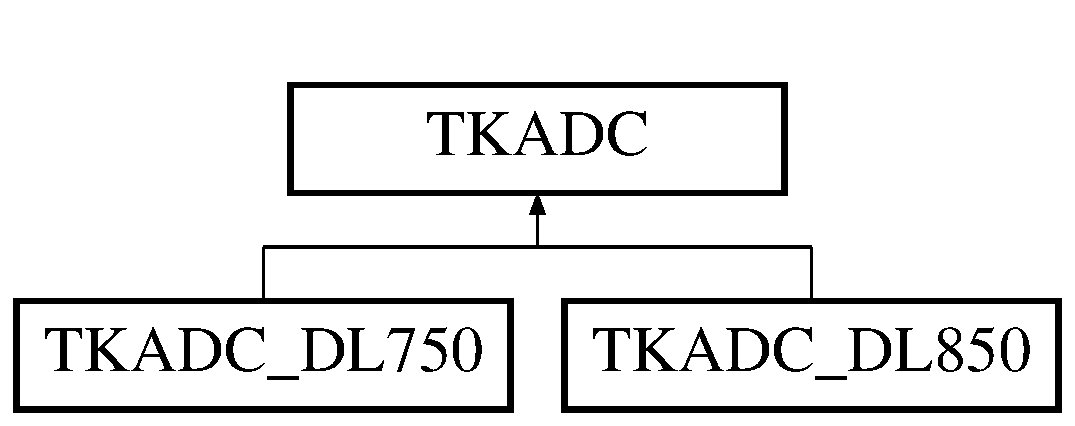
\includegraphics[height=2.000000cm]{class_t_k_a_d_c}
\end{center}
\end{figure}
\subsection*{公開型}
\begin{DoxyCompactItemize}
\item 
\mbox{\Hypertarget{class_t_k_a_d_c_a0d4ad86996884e94810d3de388fb7b35}\label{class_t_k_a_d_c_a0d4ad86996884e94810d3de388fb7b35}} 
enum {\bfseries A\+D\+C\+Model} \{ {\bfseries A\+D\+C\+Type\+D\+L750}, 
{\bfseries A\+D\+C\+Type\+D\+L850}
 \}
\item 
\mbox{\Hypertarget{class_t_k_a_d_c_ac27c023a4beb7d736056653dd395744a}\label{class_t_k_a_d_c_ac27c023a4beb7d736056653dd395744a}} 
enum {\bfseries Condition\+Flag} \{ {\bfseries A\+LL} = 0xffff
 \}
\end{DoxyCompactItemize}
\subsection*{公開メンバ関数}
\begin{DoxyCompactItemize}
\item 
\mbox{\Hypertarget{class_t_k_a_d_c_a1c0a93b410e2803b620b58a68602ddb8}\label{class_t_k_a_d_c_a1c0a93b410e2803b620b58a68602ddb8}} 
{\bfseries T\+K\+A\+DC} (A\+D\+C\+Model adcmodel)
\item 
\mbox{\Hypertarget{class_t_k_a_d_c_ae9f969478ee09be58f48b2acaca6b18e}\label{class_t_k_a_d_c_ae9f969478ee09be58f48b2acaca6b18e}} 
A\+D\+C\+Model {\bfseries Model} ()
\item 
\mbox{\Hypertarget{class_t_k_a_d_c_a325adb86439b5b155b5d39fe6bbccdd3}\label{class_t_k_a_d_c_a325adb86439b5b155b5d39fe6bbccdd3}} 
int {\bfseries Open} (int wire\+\_\+type\+\_\+, const char $\ast$adress\+\_\+)
\item 
\mbox{\Hypertarget{class_t_k_a_d_c_a35b9419768e76a1e2ae038490276fd54}\label{class_t_k_a_d_c_a35b9419768e76a1e2ae038490276fd54}} 
int {\bfseries Close} ()
\item 
\mbox{\Hypertarget{class_t_k_a_d_c_a263c827670741ec9346bab57dd2014b5}\label{class_t_k_a_d_c_a263c827670741ec9346bab57dd2014b5}} 
int {\bfseries Send\+Message} (const char $\ast$message)
\item 
\mbox{\Hypertarget{class_t_k_a_d_c_a3a72fc4842cf2d631a2125bc0a44e8b8}\label{class_t_k_a_d_c_a3a72fc4842cf2d631a2125bc0a44e8b8}} 
int {\bfseries Start} ()
\item 
\mbox{\Hypertarget{class_t_k_a_d_c_a15e1a4d09c33442b8493c55d4bdcb46e}\label{class_t_k_a_d_c_a15e1a4d09c33442b8493c55d4bdcb46e}} 
int {\bfseries Stop} ()
\item 
\mbox{\Hypertarget{class_t_k_a_d_c_a756ea455d92a0ff748471319f00802f7}\label{class_t_k_a_d_c_a756ea455d92a0ff748471319f00802f7}} 
int {\bfseries Wait\+A\+DC} ()
\item 
\mbox{\Hypertarget{class_t_k_a_d_c_a4fcfd8a9e1a211a45146b06b4fe5e62f}\label{class_t_k_a_d_c_a4fcfd8a9e1a211a45146b06b4fe5e62f}} 
int {\bfseries Wait\+A\+DC} (T\+K\+A\+D\+C\+::\+Condition\+Flag flag)
\item 
\mbox{\Hypertarget{class_t_k_a_d_c_a203501518ba49a7595572c5295d754ed}\label{class_t_k_a_d_c_a203501518ba49a7595572c5295d754ed}} 
int {\bfseries Save\+Shot} (std\+::string file\+\_\+name)
\item 
\mbox{\Hypertarget{class_t_k_a_d_c_a36ba7240885559c96262c0e85dcd5731}\label{class_t_k_a_d_c_a36ba7240885559c96262c0e85dcd5731}} 
int {\bfseries Get\+Device\+ID} ()
\item 
\mbox{\Hypertarget{class_t_k_a_d_c_af97c5fe3c01c209e154362e9dff27516}\label{class_t_k_a_d_c_af97c5fe3c01c209e154362e9dff27516}} 
virtual int {\bfseries Get\+Status\+Condition} (T\+K\+A\+D\+C\+::\+Condition\+Flag flag=Condition\+Flag\+::\+A\+LL)
\item 
\mbox{\Hypertarget{class_t_k_a_d_c_a341d18580fbda1d2e2fc9a701c16d9bf}\label{class_t_k_a_d_c_a341d18580fbda1d2e2fc9a701c16d9bf}} 
virtual int {\bfseries Delete} (std\+::string file\+\_\+name)
\item 
\mbox{\Hypertarget{class_t_k_a_d_c_a05193b85e821bec540ed791bfe82e44e}\label{class_t_k_a_d_c_a05193b85e821bec540ed791bfe82e44e}} 
int {\bfseries Get\+Last\+Local\+Shot\+Number} ()
\item 
\mbox{\Hypertarget{class_t_k_a_d_c_a7b9b8489b91d83c871b668ea64270c94}\label{class_t_k_a_d_c_a7b9b8489b91d83c871b668ea64270c94}} 
int {\bfseries Get\+Next\+Local\+Shot\+Number} ()
\item 
\mbox{\Hypertarget{class_t_k_a_d_c_ae851f7ca77f99481728881fb93576ae0}\label{class_t_k_a_d_c_ae851f7ca77f99481728881fb93576ae0}} 
int {\bfseries Set\+Last\+Local\+Shot\+Number} (int new\+\_\+local\+\_\+shot\+\_\+number)
\item 
\mbox{\Hypertarget{class_t_k_a_d_c_af3a90b165c7007a26d3ea8869970745a}\label{class_t_k_a_d_c_af3a90b165c7007a26d3ea8869970745a}} 
int {\bfseries Increment\+Local\+Shot\+Number} ()
\item 
\mbox{\Hypertarget{class_t_k_a_d_c_aa4145e024d074942bfd85777a0419cec}\label{class_t_k_a_d_c_aa4145e024d074942bfd85777a0419cec}} 
int {\bfseries Set\+Local\+Shot\+Number\+Max} (int new\+\_\+local\+\_\+shot\+\_\+number\+\_\+max)
\item 
\mbox{\Hypertarget{class_t_k_a_d_c_aa238169ef582140e6c19f84003915d87}\label{class_t_k_a_d_c_aa238169ef582140e6c19f84003915d87}} 
int {\bfseries Get\+Local\+Shot\+Number\+Max} ()
\end{DoxyCompactItemize}


このクラス詳解は次のファイルから抽出されました\+:\begin{DoxyCompactItemize}
\item 
tkadc.\+h\item 
tkadc.\+cpp\end{DoxyCompactItemize}

\hypertarget{class_t_k_a_d_c___d_l750}{}\section{T\+K\+A\+D\+C\+\_\+\+D\+L750 クラス}
\label{class_t_k_a_d_c___d_l750}\index{T\+K\+A\+D\+C\+\_\+\+D\+L750@{T\+K\+A\+D\+C\+\_\+\+D\+L750}}
T\+K\+A\+D\+C\+\_\+\+D\+L750 の継承関係図\begin{figure}[H]
\begin{center}
\leavevmode
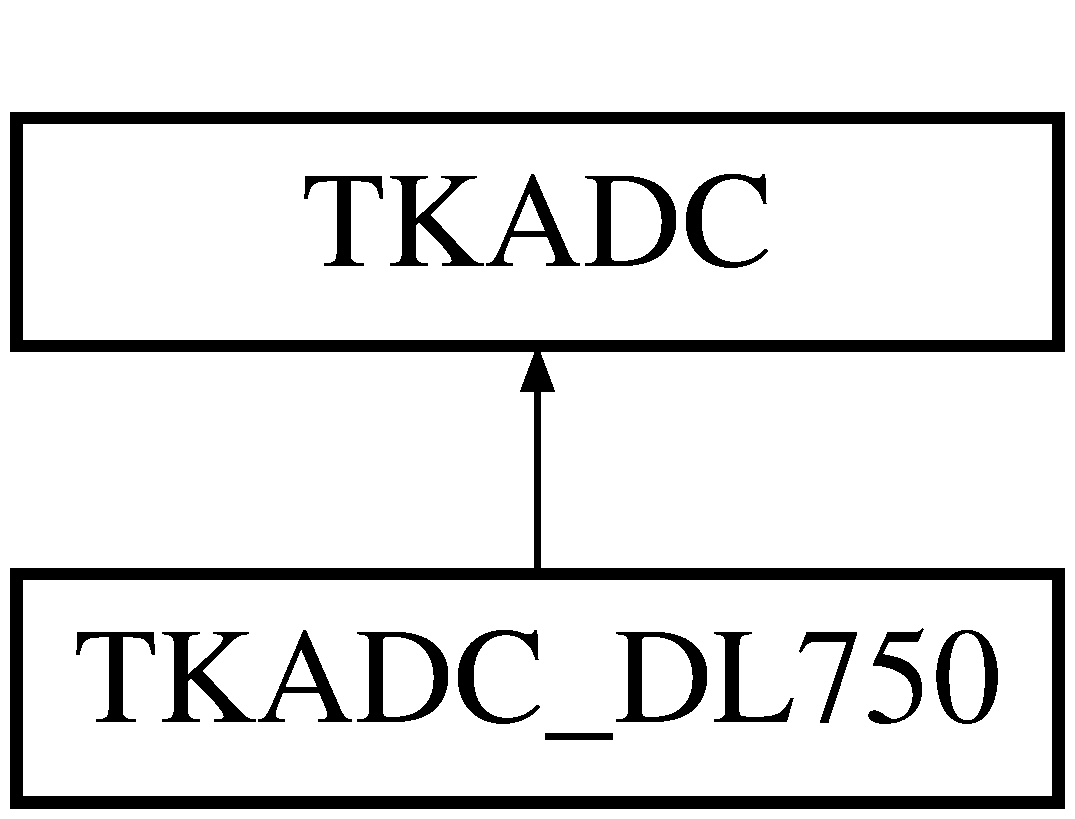
\includegraphics[height=2.000000cm]{class_t_k_a_d_c___d_l750}
\end{center}
\end{figure}
\subsection*{公開型}
\begin{DoxyCompactItemize}
\item 
\mbox{\Hypertarget{class_t_k_a_d_c___d_l750_ad5e6efe75dfb6d580542cc4843312c25}\label{class_t_k_a_d_c___d_l750_ad5e6efe75dfb6d580542cc4843312c25}} 
enum {\bfseries Condition\+Flag} \{ \newline
{\bfseries A\+LL} = 0xffff, 
{\bfseries R\+UN} = 1 $<$$<$ 0, 
{\bfseries T\+RG} = 1 $<$$<$ 2, 
{\bfseries T\+R\+G\+I\+NV} = A\+LL -\/ T\+RG, 
\newline
{\bfseries C\+AL} = 1 $<$$<$ 3, 
{\bfseries T\+ST} = 1 $<$$<$ 4, 
{\bfseries P\+RN} = 1 $<$$<$ 5, 
{\bfseries A\+CS} = 1 $<$$<$ 6, 
\newline
{\bfseries M\+ES} = 1 $<$$<$ 7, 
{\bfseries H\+ST} = 1 $<$$<$ 8, 
{\bfseries S\+UP} = 1 $<$$<$ 9, 
{\bfseries N\+GO} = 1 $<$$<$ 10, 
\newline
{\bfseries S\+CH} = 1 $<$$<$ 11, 
{\bfseries N\+SS} = 1 $<$$<$ 12, 
{\bfseries I\+NI} = 1 $<$$<$ 13, 
{\bfseries F\+FT} = 1 $<$$<$ 14
 \}
\end{DoxyCompactItemize}
\subsection*{公開メンバ関数}
\begin{DoxyCompactItemize}
\item 
\mbox{\Hypertarget{class_t_k_a_d_c___d_l750_a55a20539b69f9458422818a27ad08321}\label{class_t_k_a_d_c___d_l750_a55a20539b69f9458422818a27ad08321}} 
int {\bfseries Get\+Status\+Condition} (T\+K\+A\+D\+C\+\_\+\+D\+L750\+::\+Condition\+Flag flag=Condition\+Flag\+::\+A\+LL)
\item 
\mbox{\Hypertarget{class_t_k_a_d_c___d_l750_a7f1e774f28694761a8086797459c1b4f}\label{class_t_k_a_d_c___d_l750_a7f1e774f28694761a8086797459c1b4f}} 
int {\bfseries Delete} (std\+::string file\+\_\+name)
\end{DoxyCompactItemize}


このクラス詳解は次のファイルから抽出されました\+:\begin{DoxyCompactItemize}
\item 
tkadc.\+h\item 
tkadc.\+cpp\end{DoxyCompactItemize}

\hypertarget{class_t_k_a_d_c___d_l850}{}\section{T\+K\+A\+D\+C\+\_\+\+D\+L850 クラス}
\label{class_t_k_a_d_c___d_l850}\index{T\+K\+A\+D\+C\+\_\+\+D\+L850@{T\+K\+A\+D\+C\+\_\+\+D\+L850}}
T\+K\+A\+D\+C\+\_\+\+D\+L850 の継承関係図\begin{figure}[H]
\begin{center}
\leavevmode
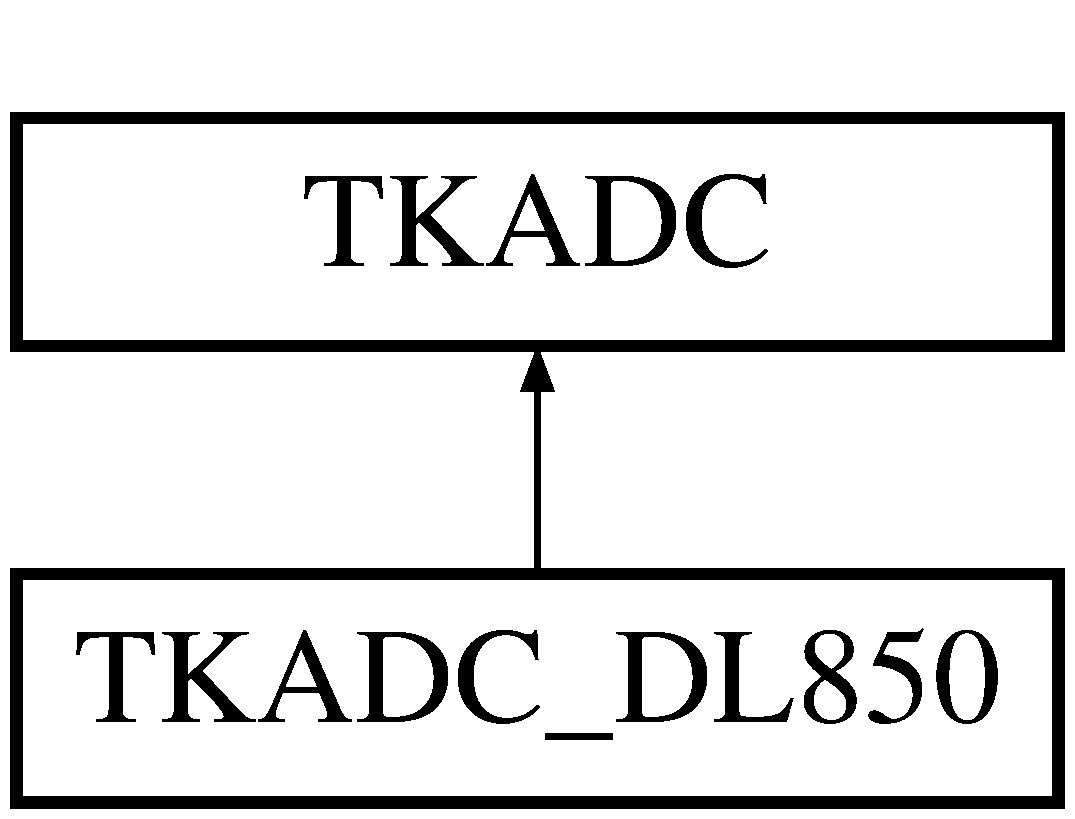
\includegraphics[height=2.000000cm]{class_t_k_a_d_c___d_l850}
\end{center}
\end{figure}
\subsection*{公開型}
\begin{DoxyCompactItemize}
\item 
\mbox{\Hypertarget{class_t_k_a_d_c___d_l850_a25f41a7cd5213cd9814195b3d6ba11c0}\label{class_t_k_a_d_c___d_l850_a25f41a7cd5213cd9814195b3d6ba11c0}} 
enum {\bfseries Condition\+Flag} \{ \newline
{\bfseries A\+LL} = 0xffff, 
{\bfseries C\+AP} = 1 $<$$<$ 0, 
{\bfseries R\+EC} = 1 $<$$<$ 1, 
{\bfseries T\+RG} = 1 $<$$<$ 2, 
\newline
{\bfseries T\+R\+G\+I\+NV} = A\+LL -\/ T\+RG, 
{\bfseries C\+AL} = 1 $<$$<$ 3, 
{\bfseries T\+ST} = 1 $<$$<$ 4, 
{\bfseries P\+RN} = 1 $<$$<$ 5, 
\newline
{\bfseries A\+CS} = 1 $<$$<$ 6, 
{\bfseries M\+ES} = 1 $<$$<$ 7, 
{\bfseries H\+ST} = 1 $<$$<$ 8, 
{\bfseries C\+NT} = 1 $<$$<$ 9, 
\newline
{\bfseries N\+GO} = 1 $<$$<$ 10, 
{\bfseries S\+CH} = 1 $<$$<$ 11, 
{\bfseries R\+UN} = 1 $<$$<$ 12, 
{\bfseries K\+LK} = 1 $<$$<$ 13, 
\newline
{\bfseries AN} = 1 $<$$<$ 14
 \}
\end{DoxyCompactItemize}
\subsection*{公開メンバ関数}
\begin{DoxyCompactItemize}
\item 
\mbox{\Hypertarget{class_t_k_a_d_c___d_l850_a1eedebd8024beb6739c598e4970e6675}\label{class_t_k_a_d_c___d_l850_a1eedebd8024beb6739c598e4970e6675}} 
int {\bfseries Get\+Status\+Condition} (T\+K\+A\+D\+C\+\_\+\+D\+L850\+::\+Condition\+Flag flag=Condition\+Flag\+::\+A\+LL)
\item 
\mbox{\Hypertarget{class_t_k_a_d_c___d_l850_a209a0e5f4c6e61a7eb3ea21a15204a7c}\label{class_t_k_a_d_c___d_l850_a209a0e5f4c6e61a7eb3ea21a15204a7c}} 
int {\bfseries Delete} (std\+::string file\+\_\+name)
\end{DoxyCompactItemize}


このクラス詳解は次のファイルから抽出されました\+:\begin{DoxyCompactItemize}
\item 
tkadc.\+h\item 
tkadc.\+cpp\end{DoxyCompactItemize}

\hypertarget{class_t_k_a_n_a_l_y_z_e_s_p}{}\section{T\+K\+A\+N\+A\+L\+Y\+Z\+E\+SP クラス}
\label{class_t_k_a_n_a_l_y_z_e_s_p}\index{T\+K\+A\+N\+A\+L\+Y\+Z\+E\+SP@{T\+K\+A\+N\+A\+L\+Y\+Z\+E\+SP}}
\subsection*{公開メンバ関数}
\begin{DoxyCompactItemize}
\item 
\mbox{\Hypertarget{class_t_k_a_n_a_l_y_z_e_s_p_aa2f68f6edb8adf34b6076f6826d56da8}\label{class_t_k_a_n_a_l_y_z_e_s_p_aa2f68f6edb8adf34b6076f6826d56da8}} 
{\bfseries T\+K\+A\+N\+A\+L\+Y\+Z\+E\+SP} (\hyperlink{class_t_k_s_h_o_t}{T\+K\+S\+H\+OT} $\ast$T\+K\+Shot\+\_\+, clx\+::ini $\ast$Setting\+\_\+)
\item 
\mbox{\Hypertarget{class_t_k_a_n_a_l_y_z_e_s_p_a1ba818f18587dca67f006dddcf38c774}\label{class_t_k_a_n_a_l_y_z_e_s_p_a1ba818f18587dca67f006dddcf38c774}} 
int {\bfseries Plot\+Raw} (T\+K\+P\+L\+O\+T\+::\+P\+L\+O\+T\+S\+I\+ZE plot\+\_\+size, int shot\+\_\+number)
\item 
\mbox{\Hypertarget{class_t_k_a_n_a_l_y_z_e_s_p_a287e554a4aee42c9232fe0d8b37f4fcb}\label{class_t_k_a_n_a_l_y_z_e_s_p_a287e554a4aee42c9232fe0d8b37f4fcb}} 
std\+::vector$<$ \hyperlink{struct_t_k_p_l_o_t_1_1_p_l_o_t_i_n_f_o}{T\+K\+P\+L\+O\+T\+::\+P\+L\+O\+T\+I\+N\+FO} $>$ {\bfseries Get\+Plot\+Info} ()
\item 
\mbox{\Hypertarget{class_t_k_a_n_a_l_y_z_e_s_p_ade64a95057a2325f7d210ee554ff5779}\label{class_t_k_a_n_a_l_y_z_e_s_p_ade64a95057a2325f7d210ee554ff5779}} 
std\+::vector$<$ \hyperlink{struct_t_k_p_l_o_t_1_1_p_l_o_t_i_n_f_o}{T\+K\+P\+L\+O\+T\+::\+P\+L\+O\+T\+I\+N\+FO} $>$\+::pointer {\bfseries Get\+Plot\+Info\+Ptr} ()
\end{DoxyCompactItemize}


このクラス詳解は次のファイルから抽出されました\+:\begin{DoxyCompactItemize}
\item 
tkanalyzesp.\+h\end{DoxyCompactItemize}

\hypertarget{class_t_k_d_a_t_a}{}\section{T\+K\+D\+A\+TA クラス}
\label{class_t_k_d_a_t_a}\index{T\+K\+D\+A\+TA@{T\+K\+D\+A\+TA}}
\subsection*{公開型}
\begin{DoxyCompactItemize}
\item 
\mbox{\Hypertarget{class_t_k_d_a_t_a_ab55f2c2d1c76bbeb3c1820ad2e749f38}\label{class_t_k_d_a_t_a_ab55f2c2d1c76bbeb3c1820ad2e749f38}} 
enum {\bfseries B\+Y\+T\+E\+O\+R\+D\+ER} \{ {\bfseries B\+I\+G\+\_\+\+E\+N\+D\+I\+AN}, 
{\bfseries L\+I\+T\+T\+L\+E\+\_\+\+E\+N\+D\+I\+AN}
 \}
\item 
\mbox{\Hypertarget{class_t_k_d_a_t_a_add3f58dbf65c97f4c9998e3a8b3f79fd}\label{class_t_k_d_a_t_a_add3f58dbf65c97f4c9998e3a8b3f79fd}} 
enum {\bfseries D\+A\+T\+A\+F\+O\+R\+M\+AT} \{ {\bfseries T\+R\+A\+CE}, 
{\bfseries B\+L\+O\+CK}
 \}
\end{DoxyCompactItemize}
\subsection*{公開メンバ関数}
\begin{DoxyCompactItemize}
\item 
\mbox{\Hypertarget{class_t_k_d_a_t_a_ad142911ef868b94bd2607ab4ca69f84d}\label{class_t_k_d_a_t_a_ad142911ef868b94bd2607ab4ca69f84d}} 
int {\bfseries Parse\+H\+DR} ()
\item 
\mbox{\Hypertarget{class_t_k_d_a_t_a_a64f288a761012bf276a5aa7f74dfcb44}\label{class_t_k_d_a_t_a_a64f288a761012bf276a5aa7f74dfcb44}} 
int {\bfseries Set\+A\+D\+C\+ID} (int iadc\+\_\+id)
\item 
\mbox{\Hypertarget{class_t_k_d_a_t_a_ad0a8defdf8de2ef2bbe42d7d8a53e051}\label{class_t_k_d_a_t_a_ad0a8defdf8de2ef2bbe42d7d8a53e051}} 
int {\bfseries Get\+A\+D\+C\+ID} ()
\item 
\mbox{\Hypertarget{class_t_k_d_a_t_a_ae63b673fda97ff6fef659f51fe40dbe8}\label{class_t_k_d_a_t_a_ae63b673fda97ff6fef659f51fe40dbe8}} 
int {\bfseries Set\+Data\+File\+Name} (std\+::string idata\+\_\+file\+\_\+name)
\item 
\mbox{\Hypertarget{class_t_k_d_a_t_a_a3f354a0eb29025867cbd1e3e27f8e41a}\label{class_t_k_d_a_t_a_a3f354a0eb29025867cbd1e3e27f8e41a}} 
std\+::string {\bfseries Get\+Data\+File\+Name} ()
\item 
\mbox{\Hypertarget{class_t_k_d_a_t_a_a0f0c38948586490c1bfe1f820418c5ef}\label{class_t_k_d_a_t_a_a0f0c38948586490c1bfe1f820418c5ef}} 
float {\bfseries Get\+H\+Resolution} ()
\item 
\mbox{\Hypertarget{class_t_k_d_a_t_a_a6c83babefbef168db08ca1c00cfe560d}\label{class_t_k_d_a_t_a_a6c83babefbef168db08ca1c00cfe560d}} 
float {\bfseries Get\+V\+Offset} (int const trace\+\_\+index)
\item 
\mbox{\Hypertarget{class_t_k_d_a_t_a_a78fccdabf4c7326ecb9dbe30ebe765e4}\label{class_t_k_d_a_t_a_a78fccdabf4c7326ecb9dbe30ebe765e4}} 
float {\bfseries Get\+V\+Resolution} (int const trace\+\_\+index)
\item 
\mbox{\Hypertarget{class_t_k_d_a_t_a_aaa91499a0c86542c6d240f07b2c7a5a6}\label{class_t_k_d_a_t_a_aaa91499a0c86542c6d240f07b2c7a5a6}} 
int {\bfseries Get\+V\+Max\+Data} (int const trace\+\_\+index)
\item 
\mbox{\Hypertarget{class_t_k_d_a_t_a_aed38093c0f7a086ab190c89770567531}\label{class_t_k_d_a_t_a_aed38093c0f7a086ab190c89770567531}} 
int {\bfseries Get\+V\+Min\+Data} (int const trace\+\_\+index)
\item 
\mbox{\Hypertarget{class_t_k_d_a_t_a_a5fe237cba051e352845786e13c0cd54f}\label{class_t_k_d_a_t_a_a5fe237cba051e352845786e13c0cd54f}} 
int {\bfseries Get\+Block\+Size} ()
\item 
\mbox{\Hypertarget{class_t_k_d_a_t_a_ac823854fcfb02d7788ec491b38f4d615}\label{class_t_k_d_a_t_a_ac823854fcfb02d7788ec491b38f4d615}} 
float {\bfseries Get\+H\+Offset} ()
\item 
\mbox{\Hypertarget{class_t_k_d_a_t_a_af0a676448ec4d492290517a7e60a2de3}\label{class_t_k_d_a_t_a_af0a676448ec4d492290517a7e60a2de3}} 
std\+::string {\bfseries Get\+Model\+Name} ()
\item 
\mbox{\Hypertarget{class_t_k_d_a_t_a_a63437cd1b2448b0b54ee6ec56da1321e}\label{class_t_k_d_a_t_a_a63437cd1b2448b0b54ee6ec56da1321e}} 
T\+K\+D\+A\+T\+A\+::\+B\+Y\+T\+E\+O\+R\+D\+ER {\bfseries Get\+Byte\+Order} ()
\item 
\mbox{\Hypertarget{class_t_k_d_a_t_a_a86117b4edecbf2e3013973fb016877e2}\label{class_t_k_d_a_t_a_a86117b4edecbf2e3013973fb016877e2}} 
T\+K\+D\+A\+T\+A\+::\+D\+A\+T\+A\+F\+O\+R\+M\+AT {\bfseries Get\+Data\+Format} ()
\item 
\mbox{\Hypertarget{class_t_k_d_a_t_a_a11fad512e15a5b8dd7be2ff786d5fd8e}\label{class_t_k_d_a_t_a_a11fad512e15a5b8dd7be2ff786d5fd8e}} 
int {\bfseries Get\+Data\+Offset} ()
\item 
\mbox{\Hypertarget{class_t_k_d_a_t_a_a0e9270376ed47917048fdd38f2f4a81d}\label{class_t_k_d_a_t_a_a0e9270376ed47917048fdd38f2f4a81d}} 
int {\bfseries Get\+Trace\+Total\+Number} ()
\item 
\mbox{\Hypertarget{class_t_k_d_a_t_a_ad70108b9612759566d7cc90e60f293c5}\label{class_t_k_d_a_t_a_ad70108b9612759566d7cc90e60f293c5}} 
int {\bfseries Channnel\+Number\+To\+Trace\+Number} (int const channel\+\_\+number)
\item 
\mbox{\Hypertarget{class_t_k_d_a_t_a_a8282e57fcee3618dfe533b6771adce96}\label{class_t_k_d_a_t_a_a8282e57fcee3618dfe533b6771adce96}} 
int {\bfseries Get\+Channel\+Number} (int const trace\+\_\+index)
\end{DoxyCompactItemize}


このクラス詳解は次のファイルから抽出されました\+:\begin{DoxyCompactItemize}
\item 
U\+I/\+Project1/tkshotinfo.\+h\item 
U\+I/\+Project1/tkshotinfo.\+cpp\end{DoxyCompactItemize}

\hypertarget{class_t_k_particle_palameter}{}\section{T\+K\+Particle\+Palameter クラス}
\label{class_t_k_particle_palameter}\index{T\+K\+Particle\+Palameter@{T\+K\+Particle\+Palameter}}
\subsection*{公開変数類}
\begin{DoxyCompactItemize}
\item 
\mbox{\Hypertarget{class_t_k_particle_palameter_a23ae16244a4143ee0642cf6620facf31}\label{class_t_k_particle_palameter_a23ae16244a4143ee0642cf6620facf31}} 
double {\bfseries density}
\item 
\mbox{\Hypertarget{class_t_k_particle_palameter_a65c396039f6aaf454837c2139af9da65}\label{class_t_k_particle_palameter_a65c396039f6aaf454837c2139af9da65}} 
double {\bfseries temperature}
\item 
\mbox{\Hypertarget{class_t_k_particle_palameter_a9be89d1ba1cb6c97e6154bf9f91f2437}\label{class_t_k_particle_palameter_a9be89d1ba1cb6c97e6154bf9f91f2437}} 
double {\bfseries mass}
\end{DoxyCompactItemize}


このクラス詳解は次のファイルから抽出されました\+:\begin{DoxyCompactItemize}
\item 
U\+I/\+Project1/tkphysics.\+h\end{DoxyCompactItemize}

\hypertarget{class_t_k_plasma}{}\section{T\+K\+Plasma クラス}
\label{class_t_k_plasma}\index{T\+K\+Plasma@{T\+K\+Plasma}}
\subsection*{公開変数類}
\begin{DoxyCompactItemize}
\item 
\mbox{\Hypertarget{class_t_k_plasma_ab2ba31fba9c3b255fa454d557b46c552}\label{class_t_k_plasma_ab2ba31fba9c3b255fa454d557b46c552}} 
double const  \& {\bfseries n\+\_\+e} = electron.\+density
\item 
\mbox{\Hypertarget{class_t_k_plasma_af742f3b64a9c48f6f0e3184bf7ebb0c2}\label{class_t_k_plasma_af742f3b64a9c48f6f0e3184bf7ebb0c2}} 
double const  \& {\bfseries n\+\_\+n} = neutral.\+density
\item 
\mbox{\Hypertarget{class_t_k_plasma_a0074fb0c178f69de84d5509d0bfd4ac0}\label{class_t_k_plasma_a0074fb0c178f69de84d5509d0bfd4ac0}} 
double const {\bfseries a}
\end{DoxyCompactItemize}


このクラス詳解は次のファイルから抽出されました\+:\begin{DoxyCompactItemize}
\item 
tkphysics.\+h\end{DoxyCompactItemize}

\hypertarget{class_t_k_plasma_parameter}{}\section{T\+K\+Plasma\+Parameter クラス}
\label{class_t_k_plasma_parameter}\index{T\+K\+Plasma\+Parameter@{T\+K\+Plasma\+Parameter}}


このクラス詳解は次のファイルから抽出されました\+:\begin{DoxyCompactItemize}
\item 
U\+I/\+Project1/tkphysics.\+h\end{DoxyCompactItemize}

\hypertarget{class_t_k_p_l_o_t}{}\section{T\+K\+P\+L\+OT クラス}
\label{class_t_k_p_l_o_t}\index{T\+K\+P\+L\+OT@{T\+K\+P\+L\+OT}}


{\ttfamily \#include $<$tkplot.\+h$>$}

T\+K\+P\+L\+OT の継承関係図\begin{figure}[H]
\begin{center}
\leavevmode
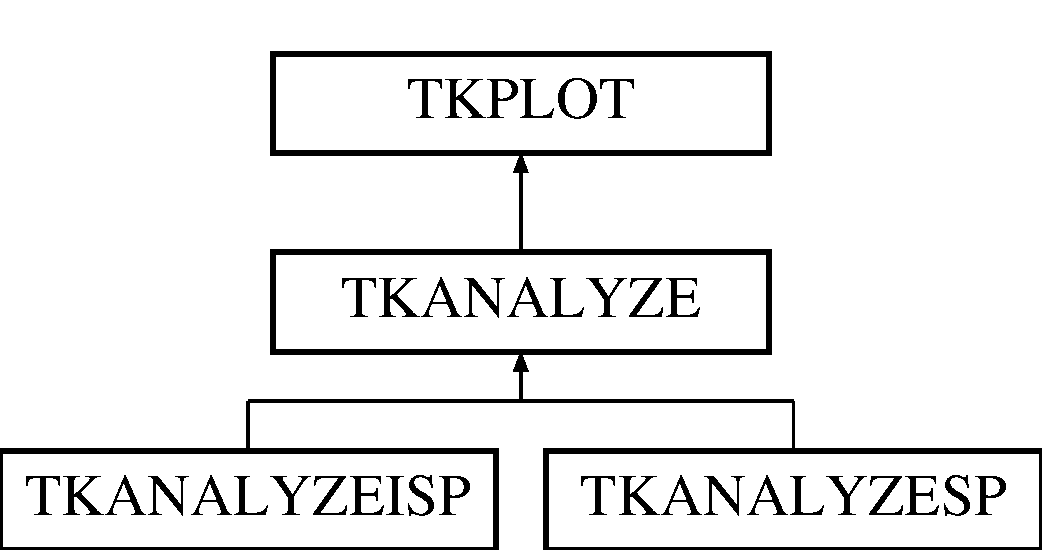
\includegraphics[height=3.000000cm]{class_t_k_p_l_o_t}
\end{center}
\end{figure}
\subsection*{クラス}
\begin{DoxyCompactItemize}
\item 
class \hyperlink{class_t_k_p_l_o_t_1_1_p_l_o_t_i_n_f_o}{P\+L\+O\+T\+I\+N\+FO}
\item 
class \hyperlink{class_t_k_p_l_o_t_1_1_p_o_s_i_t_i_o_n}{P\+O\+S\+I\+T\+I\+ON}
\item 
class \hyperlink{class_t_k_p_l_o_t_1_1_r_a_n_g_e}{R\+A\+N\+GE}
\item 
class \hyperlink{class_t_k_p_l_o_t_1_1_s_i_z_e}{S\+I\+ZE}
\end{DoxyCompactItemize}
\subsection*{公開型}
\begin{DoxyCompactItemize}
\item 
enum \hyperlink{class_t_k_p_l_o_t_a158082ae168750554cf23edde9a27416}{P\+L\+O\+T\+S\+I\+ZE} \{ {\bfseries S\+M\+A\+L\+L\+\_\+\+S\+I\+ZE}, 
{\bfseries M\+E\+D\+I\+U\+M\+\_\+\+S\+I\+ZE}
 \}
\item 
enum \hyperlink{class_t_k_p_l_o_t_a28dfea1dd78dfc49c1926518da615bfa}{D\+A\+T\+A\+S\+O\+U\+R\+CE} \{ \hyperlink{class_t_k_p_l_o_t_a28dfea1dd78dfc49c1926518da615bfaa98ad0e8750ae10ad556ed7a62affb452}{D\+A\+T\+A\+S\+O\+U\+R\+C\+E\+::\+B\+I\+N\+A\+RY}, 
\hyperlink{class_t_k_p_l_o_t_a28dfea1dd78dfc49c1926518da615bfaad2cd8253361a9c732d21ca1d336599cc}{D\+A\+T\+A\+S\+O\+U\+R\+C\+E\+::\+A\+S\+C\+II}
 \}
\end{DoxyCompactItemize}
\subsection*{公開メンバ関数}
\begin{DoxyCompactItemize}
\item 
\mbox{\Hypertarget{class_t_k_p_l_o_t_aeb9168bcf7e45c45fc38dab63e6b90b3}\label{class_t_k_p_l_o_t_aeb9168bcf7e45c45fc38dab63e6b90b3}} 
{\bfseries T\+K\+P\+L\+OT} (\hyperlink{class_t_k_s_h_o_t}{T\+K\+S\+H\+OT} $\ast$T\+K\+Shot\+\_\+)
\item 
\mbox{\Hypertarget{class_t_k_p_l_o_t_a0dcffb0672762042e8dca5791b97e182}\label{class_t_k_p_l_o_t_a0dcffb0672762042e8dca5791b97e182}} 
int {\bfseries Plot\+Raw} (const \hyperlink{class_t_k_p_l_o_t_a158082ae168750554cf23edde9a27416}{T\+K\+P\+L\+O\+T\+::\+P\+L\+O\+T\+S\+I\+ZE} plot\+\_\+size, const int shot\+\_\+number, bool replot=true)
\item 
\mbox{\Hypertarget{class_t_k_p_l_o_t_a5ddc4ef2a68d8649cfb2aebf507121fd}\label{class_t_k_p_l_o_t_a5ddc4ef2a68d8649cfb2aebf507121fd}} 
std\+::vector$<$ \hyperlink{class_t_k_p_l_o_t_1_1_p_l_o_t_i_n_f_o}{T\+K\+P\+L\+O\+T\+::\+P\+L\+O\+T\+I\+N\+FO} $>$ {\bfseries Get\+Plot\+Info} ()
\item 
\mbox{\Hypertarget{class_t_k_p_l_o_t_a4087cc1a73e760ac8eb32cbdf78a4433}\label{class_t_k_p_l_o_t_a4087cc1a73e760ac8eb32cbdf78a4433}} 
std\+::vector$<$ \hyperlink{class_t_k_p_l_o_t_1_1_p_l_o_t_i_n_f_o}{T\+K\+P\+L\+O\+T\+::\+P\+L\+O\+T\+I\+N\+FO} $>$\+::pointer {\bfseries Get\+Plot\+Info\+Ptr} ()
\end{DoxyCompactItemize}
\subsection*{限定公開メンバ関数}
\begin{DoxyCompactItemize}
\item 
\mbox{\Hypertarget{class_t_k_p_l_o_t_aae92c92917093101c52d08d132aee75b}\label{class_t_k_p_l_o_t_aae92c92917093101c52d08d132aee75b}} 
\hyperlink{class_t_k_p_l_o_t_1_1_p_l_o_t_i_n_f_o}{P\+L\+O\+T\+I\+N\+FO} \& {\bfseries load\+Plot\+Info\+Instance} (const int data\+\_\+index, const int trace\+\_\+index, const \hyperlink{class_t_k_p_l_o_t_a158082ae168750554cf23edde9a27416}{P\+L\+O\+T\+S\+I\+ZE} plot\+\_\+size=P\+L\+O\+T\+S\+I\+Z\+E\+::\+S\+M\+A\+L\+L\+\_\+\+S\+I\+ZE)
\end{DoxyCompactItemize}


\subsection{詳解}
グラフ描画に関するクラスです。 

\subsection{列挙型メンバ詳解}
\mbox{\Hypertarget{class_t_k_p_l_o_t_a28dfea1dd78dfc49c1926518da615bfa}\label{class_t_k_p_l_o_t_a28dfea1dd78dfc49c1926518da615bfa}} 
\index{T\+K\+P\+L\+OT@{T\+K\+P\+L\+OT}!D\+A\+T\+A\+S\+O\+U\+R\+CE@{D\+A\+T\+A\+S\+O\+U\+R\+CE}}
\index{D\+A\+T\+A\+S\+O\+U\+R\+CE@{D\+A\+T\+A\+S\+O\+U\+R\+CE}!T\+K\+P\+L\+OT@{T\+K\+P\+L\+OT}}
\subsubsection{\texorpdfstring{D\+A\+T\+A\+S\+O\+U\+R\+CE}{DATASOURCE}}
{\footnotesize\ttfamily enum \hyperlink{class_t_k_p_l_o_t_a28dfea1dd78dfc49c1926518da615bfa}{T\+K\+P\+L\+O\+T\+::\+D\+A\+T\+A\+S\+O\+U\+R\+CE}\hspace{0.3cm}{\ttfamily [strong]}}

データファイル形式型 \begin{DoxyEnumFields}{列挙値}
\raisebox{\heightof{T}}[0pt][0pt]{\index{B\+I\+N\+A\+RY@{B\+I\+N\+A\+RY}!T\+K\+P\+L\+OT@{T\+K\+P\+L\+OT}}\index{T\+K\+P\+L\+OT@{T\+K\+P\+L\+OT}!B\+I\+N\+A\+RY@{B\+I\+N\+A\+RY}}}\mbox{\Hypertarget{class_t_k_p_l_o_t_a28dfea1dd78dfc49c1926518da615bfaa98ad0e8750ae10ad556ed7a62affb452}\label{class_t_k_p_l_o_t_a28dfea1dd78dfc49c1926518da615bfaa98ad0e8750ae10ad556ed7a62affb452}} 
B\+I\+N\+A\+RY&バイナリファイル~\newline
 非常に高速に処理できますが、柔軟性にかけるため使用できないことがあります。 \\
\hline

\raisebox{\heightof{T}}[0pt][0pt]{\index{A\+S\+C\+II@{A\+S\+C\+II}!T\+K\+P\+L\+OT@{T\+K\+P\+L\+OT}}\index{T\+K\+P\+L\+OT@{T\+K\+P\+L\+OT}!A\+S\+C\+II@{A\+S\+C\+II}}}\mbox{\Hypertarget{class_t_k_p_l_o_t_a28dfea1dd78dfc49c1926518da615bfaad2cd8253361a9c732d21ca1d336599cc}\label{class_t_k_p_l_o_t_a28dfea1dd78dfc49c1926518da615bfaad2cd8253361a9c732d21ca1d336599cc}} 
A\+S\+C\+II&A\+S\+C\+I\+Iファイル~\newline
 データ変換のイニシャルタイムが必要であり、データ読み込みもハイコストなため、処理は遅くなりますが、全ての機能を利用できます。 \\
\hline

\end{DoxyEnumFields}
\mbox{\Hypertarget{class_t_k_p_l_o_t_a158082ae168750554cf23edde9a27416}\label{class_t_k_p_l_o_t_a158082ae168750554cf23edde9a27416}} 
\index{T\+K\+P\+L\+OT@{T\+K\+P\+L\+OT}!P\+L\+O\+T\+S\+I\+ZE@{P\+L\+O\+T\+S\+I\+ZE}}
\index{P\+L\+O\+T\+S\+I\+ZE@{P\+L\+O\+T\+S\+I\+ZE}!T\+K\+P\+L\+OT@{T\+K\+P\+L\+OT}}
\subsubsection{\texorpdfstring{P\+L\+O\+T\+S\+I\+ZE}{PLOTSIZE}}
{\footnotesize\ttfamily enum \hyperlink{class_t_k_p_l_o_t_a158082ae168750554cf23edde9a27416}{T\+K\+P\+L\+O\+T\+::\+P\+L\+O\+T\+S\+I\+ZE}\hspace{0.3cm}{\ttfamily [strong]}}

グラフサイズ型 

このクラス詳解は次のファイルから抽出されました\+:\begin{DoxyCompactItemize}
\item 
tkplot.\+h\end{DoxyCompactItemize}

\hypertarget{class_t_k_s_h_o_t}{}\section{T\+K\+S\+H\+OT クラス}
\label{class_t_k_s_h_o_t}\index{T\+K\+S\+H\+OT@{T\+K\+S\+H\+OT}}
\subsection*{公開メンバ関数}
\begin{DoxyCompactItemize}
\item 
\mbox{\Hypertarget{class_t_k_s_h_o_t_af116d5e195d9853c78d3e4ddb00e2c57}\label{class_t_k_s_h_o_t_af116d5e195d9853c78d3e4ddb00e2c57}} 
int {\bfseries Get\+A\+D\+C\+Number} ()
\item 
\mbox{\Hypertarget{class_t_k_s_h_o_t_a1314067d1c3ec702c29866ad124048eb}\label{class_t_k_s_h_o_t_a1314067d1c3ec702c29866ad124048eb}} 
std\+::string {\bfseries Get\+Data\+File\+Name} (int adc\+\_\+id)
\item 
\mbox{\Hypertarget{class_t_k_s_h_o_t_a8f91dff3640a574152c6fb3c5e542f62}\label{class_t_k_s_h_o_t_a8f91dff3640a574152c6fb3c5e542f62}} 
int {\bfseries Name\+Shot\+Number} (int ishot\+\_\+number)
\item 
\mbox{\Hypertarget{class_t_k_s_h_o_t_a8edc2c710c0dd04d619ddb5f105c41fe}\label{class_t_k_s_h_o_t_a8edc2c710c0dd04d619ddb5f105c41fe}} 
int {\bfseries Clear} ()
\item 
\mbox{\Hypertarget{class_t_k_s_h_o_t_ae8f63779c8d19ad6afab9e02ba066487}\label{class_t_k_s_h_o_t_ae8f63779c8d19ad6afab9e02ba066487}} 
int {\bfseries Append\+Data\+File} (std\+::string data\+\_\+file\+\_\+name)
\item 
\mbox{\Hypertarget{class_t_k_s_h_o_t_a055079afd19a206d3f525b6c2cbd5d75}\label{class_t_k_s_h_o_t_a055079afd19a206d3f525b6c2cbd5d75}} 
float {\bfseries Get\+H\+Resolution} (int adc\+\_\+id)
\item 
\mbox{\Hypertarget{class_t_k_s_h_o_t_abc9d569e4f7136cd0b3f56b8e0e2e8cd}\label{class_t_k_s_h_o_t_abc9d569e4f7136cd0b3f56b8e0e2e8cd}} 
int {\bfseries Get\+Block\+Size} (int adc\+\_\+id)
\item 
\mbox{\Hypertarget{class_t_k_s_h_o_t_ab43a63e3fe0f6797ee97eed0091339ba}\label{class_t_k_s_h_o_t_ab43a63e3fe0f6797ee97eed0091339ba}} 
float {\bfseries Get\+V\+Offset} (int adc\+\_\+id, int trace\+\_\+index)
\item 
\mbox{\Hypertarget{class_t_k_s_h_o_t_aafff8aa391415312187f769a4678c82f}\label{class_t_k_s_h_o_t_aafff8aa391415312187f769a4678c82f}} 
float {\bfseries Get\+V\+Resolution} (int adc\+\_\+id, int trace\+\_\+index)
\item 
\mbox{\Hypertarget{class_t_k_s_h_o_t_aa69c94f494055fd98ff3982681d6795c}\label{class_t_k_s_h_o_t_aa69c94f494055fd98ff3982681d6795c}} 
int {\bfseries Get\+V\+Max\+Data} (int adc\+\_\+id, int trace\+\_\+index)
\item 
\mbox{\Hypertarget{class_t_k_s_h_o_t_ab02def889d5bf8c6103dbac2a5f89ab6}\label{class_t_k_s_h_o_t_ab02def889d5bf8c6103dbac2a5f89ab6}} 
int {\bfseries Get\+V\+Min\+Data} (int adc\+\_\+id, int trace\+\_\+index)
\item 
\mbox{\Hypertarget{class_t_k_s_h_o_t_ae9bd114c4904e0f20929988b4307587f}\label{class_t_k_s_h_o_t_ae9bd114c4904e0f20929988b4307587f}} 
float {\bfseries Get\+H\+Offset} (int adc\+\_\+id)
\item 
\mbox{\Hypertarget{class_t_k_s_h_o_t_adb4af221e08781c6f742ff681d134163}\label{class_t_k_s_h_o_t_adb4af221e08781c6f742ff681d134163}} 
std\+::string {\bfseries Get\+Model\+Name} (int adc\+\_\+id)
\item 
\mbox{\Hypertarget{class_t_k_s_h_o_t_acfcfbf59a93120c97de2eee6acec5104}\label{class_t_k_s_h_o_t_acfcfbf59a93120c97de2eee6acec5104}} 
T\+K\+D\+A\+T\+A\+::\+B\+Y\+T\+E\+O\+R\+D\+ER {\bfseries Get\+Byte\+Order} (int adc\+\_\+id)
\item 
\mbox{\Hypertarget{class_t_k_s_h_o_t_a30ef4f11ad37a0e1ab3002d6e7a335d6}\label{class_t_k_s_h_o_t_a30ef4f11ad37a0e1ab3002d6e7a335d6}} 
T\+K\+D\+A\+T\+A\+::\+D\+A\+T\+A\+F\+O\+R\+M\+AT {\bfseries Get\+Data\+Format} (int adc\+\_\+id)
\item 
\mbox{\Hypertarget{class_t_k_s_h_o_t_ace4770ac6dcdec71ce95823689a58380}\label{class_t_k_s_h_o_t_ace4770ac6dcdec71ce95823689a58380}} 
int {\bfseries Get\+Data\+Offset} (int adc\+\_\+id)
\item 
\mbox{\Hypertarget{class_t_k_s_h_o_t_a45a19a71b5d82762601acef738ad504d}\label{class_t_k_s_h_o_t_a45a19a71b5d82762601acef738ad504d}} 
int {\bfseries Get\+Trace\+Total\+Number} (int adc\+\_\+id)
\item 
\mbox{\Hypertarget{class_t_k_s_h_o_t_a370000c7133ee68afe584d7c74864411}\label{class_t_k_s_h_o_t_a370000c7133ee68afe584d7c74864411}} 
int {\bfseries A\+D\+C\+I\+D\+To\+A\+D\+C\+Data\+Index} (int adc\+\_\+id)
\item 
\mbox{\Hypertarget{class_t_k_s_h_o_t_a5402cb531f82fe70ba46a4f0d97dfedf}\label{class_t_k_s_h_o_t_a5402cb531f82fe70ba46a4f0d97dfedf}} 
int {\bfseries Get\+A\+D\+C\+ID} (int adc\+\_\+index)
\item 
\mbox{\Hypertarget{class_t_k_s_h_o_t_a71522d246c17a4643838a01bef2943ff}\label{class_t_k_s_h_o_t_a71522d246c17a4643838a01bef2943ff}} 
int {\bfseries Get\+Channel\+Number} (int adc\+\_\+id, int trace\+\_\+index)
\end{DoxyCompactItemize}


このクラス詳解は次のファイルから抽出されました\+:\begin{DoxyCompactItemize}
\item 
tkshotinfo.\+h\end{DoxyCompactItemize}

\hypertarget{struct_project1_1_1_my_form_1_1clx_1_1detail_1_1widest__char}{}\section{Project1\+:\+:My\+Form\+:\+:clx\+:\+:detail\+:\+:widest\+\_\+char$<$ Type\+Char, Source\+Char $>$ 構造体テンプレート}
\label{struct_project1_1_1_my_form_1_1clx_1_1detail_1_1widest__char}\index{Project1\+::\+My\+Form\+::clx\+::detail\+::widest\+\_\+char$<$ Type\+Char, Source\+Char $>$@{Project1\+::\+My\+Form\+::clx\+::detail\+::widest\+\_\+char$<$ Type\+Char, Source\+Char $>$}}
\subsection*{公開型}
\begin{DoxyCompactItemize}
\item 
\mbox{\Hypertarget{struct_project1_1_1_my_form_1_1clx_1_1detail_1_1widest__char_a4aa71a0d7a47cc56ba9b8520126f8b21}\label{struct_project1_1_1_my_form_1_1clx_1_1detail_1_1widest__char_a4aa71a0d7a47cc56ba9b8520126f8b21}} 
typedef Type\+Char {\bfseries type}
\end{DoxyCompactItemize}


この構造体詳解は次のファイルから抽出されました\+:\begin{DoxyCompactItemize}
\item 
U\+I/\+Project1/My\+Form.\+h\end{DoxyCompactItemize}

%--- End generated contents ---

% Index
\backmatter
\newpage
\phantomsection
\clearemptydoublepage
\addcontentsline{toc}{chapter}{索引}
\printindex

\end{document}
